\documentclass[UTF8,a4paper,11pt,fontset=fandol]{ctexart}
\IfFontExistsTF{Droid Sans Fallback}
  {\newCJKfontfamily\cjkfallback{Droid Sans Fallback}}
  {\IfFontExistsTF{Noto Sans CJK SC}
    {\newCJKfontfamily\cjkfallback{Noto Sans CJK SC}}
    {\newcommand{\cjkfallback}{\CJKfamily{song}}}}
\usepackage[margin=22mm,headheight=15pt]{geometry}
\usepackage{graphicx,float,xcolor,amsmath,amssymb,booktabs,longtable,array,tabularx}
\usepackage[most]{tcolorbox}
\usepackage{listings,needspace,fancyhdr,enumitem}
\setlist{leftmargin=2em,itemsep=0.35em,topsep=0.4em,parsep=0pt}
\usepackage[unicode,colorlinks=true,linkcolor=blue!45!black,urlcolor=blue!45!black,breaklinks=true]{hyperref}
\usepackage{xurl}
\setlength{\parindent}{0pt}
\setlength{\parskip}{0.65em}
\setlength{\emergencystretch}{3em}
\linespread{1.14}
\raggedbottom
\pagestyle{fancy}\fancyhf{}\fancyhead[L]{硅谷101 · 访谈学习笔记}\fancyfoot[C]{\thepage}
\newtcolorbox{importantbox}[1]{enhanced,breakable,colback=blue!3,colframe=blue!45!black,title={#1},fonttitle=\bfseries}
\newtcolorbox{knowledgebox}[1]{enhanced,breakable,colback=teal!3,colframe=teal!50!black,title={#1},fonttitle=\bfseries}
\newtcolorbox{warningbox}[1]{enhanced,breakable,colback=orange!4,colframe=orange!60!black,title={#1},fonttitle=\bfseries}
\lstset{basicstyle=\ttfamily\small,breaklines=true,columns=fullflexible,keepspaces=true,showstringspaces=false,frame=single,captionpos=b}
\newcolumntype{Y}{>{\raggedright\arraybackslash}X}
\newcommand{\notetitle}{AI 时代怎样学习：大学、判断力与个人工作流}
\newcommand{\videocoverpath}{cover.jpg}
\newcommand{\videourl}{https://www.bilibili.com/video/BV1zD5a6bEoY/}
\newcommand{\videochannel}{硅谷101播客}
\newcommand{\videopublishdate}{2026-05-15}
\newcommand{\noteauthors}{泓君、林桐宇、侯泰羽、饶杰武}
\newcommand{\sourceurl}{https://www.bilibili.com/video/BV1zD5a6bEoY/}
\begin{document}

\begin{titlepage}\centering\vspace*{4mm}
{\Large 硅谷101 · 访谈学习笔记\par}\vspace{8mm}
{\LARGE\bfseries \notetitle\par}\vspace{7mm}

\includegraphics[width=.86\linewidth,height=.27\textheight,keepaspectratio]{cover.jpg}
\par\vspace{6mm}{\small 原节目：99\%的作业都是AI写的：当代名校生眼里，大学还剩下什么？【硅谷101播客】\par}
\vspace{4mm}主播：泓君\par
{\small 林桐宇 (Alfred)，清华大学法学（国际）2026届\par}
{\small 侯泰羽 (Kolento)，纽约大学应用心理学2026届\par}
{\small 饶杰武 (Jack)，哥伦比亚大学管理科学与工程研究生2026届，Emergences Labs 创始人兼CTO\par}
\vfill 录制：2026年2月\quad 发布：2026-05-15\par
整理：2026-10-20\quad 正文：Gemini Argon\quad 配图与编校：Codex\par
\vspace{4mm}\url{https://www.bilibili.com/video/BV1zD5a6bEoY/}
\end{titlepage}
\begingroup\small\setlength{\parskip}{0pt}\tableofcontents\endgroup\clearpage
\section*{导读}\addcontentsline{toc}{section}{导读}
本篇学习笔记整理自《硅谷101》播客第 2026 年 2 月录制、同年 5 月 15 日发布的圆桌访谈。主持人泓君对话三位与生成式 AI 同步走过大学时光的名校学生：清华大学法学本科生林桐宇（Alfred）、纽约大学应用心理学本科毕业生侯泰羽（Kolento），以及纽约大学数据科学本科、哥伦比亚大学管理科学与工程硕士毕业生饶杰武（Jack）。笔记围绕“大学还剩下什么”这一问题展开：从文科生跨界学编程与备考法律论述的闭环，到大学在自我认知、深度人际连接与社会信任凭证上的价值重分配；从课堂评价分化与逆向学习法，到 AI 高频参与作业时的需求拆解与人工把关；再到多模型个人工作流编排、底层能力自查，以及结合 METR 实证研究与新闻采写经验对“全链路效率”的核算，系统呈现当代学习者在与工具共处中保留判断力与主体性的实践路径。
\needspace{8\baselineskip}\section{从法律课堂到 AI 项目}
2022年底 ChatGPT 上线时，清华大学法学本科生林桐宇（Alfred）刚刚开始大一生活。当基础法律分析与文书撰写能被模型高效处理时，传统的文科训练该如何寻找出路？本章通过 Alfred 的亲身经历，拆解他如何将职业焦虑转化为学习动力，在计算机辅修与法学主修中建立“基础概念—多轮追问—项目与应试检验”的个人学习闭环。
\needspace{6\baselineskip}\subsection{职业冲击怎样变成学习问题}
对于刚进入大学的文科生来说，生成式人工智能（Generative AI，指能够根据输入提示生成文本、代码等新内容的模型）首先带来的是直接的职业危机感。主播泓君在访谈开篇将话题投向清华大学法学院本科生林桐宇（Alfred）：一名标准文科背景的学生，为什么会成为 AI 的重度使用者并跨界学习编程？Alfred 回忆，自己大一在法学主修上投入不足，平时利用空余时间辅修计算机科学（CS，研究计算系统、软件设计与算法原理的学科）。2022年底至2023年初 ChatGPT 出现后，他发现模型在特定法律条款分析和法律文书撰写上的表现已经明显超过当时的自己。由此他产生了一个紧迫的推演：两三年后毕业时，AI 的能力会继续增强，如果自己的专业水平没有实质突破，在职场上还能承担什么角色（04:06–05:08）？

这种个人危机感很快在行业资深人士那里得到了印证。2023年中，在一门由美国律所并购方向十几年资深合伙人讲授的课程结课时，Alfred 向这位任课老师提问：ChatGPT 是否会对未来的初级律师（Junior 律师，刚入行、主要负责检索与文书初稿的年轻律师）和律师助理（Paralegal，协助律师进行法规检索、案卷整理与文书准备的辅助人员）造成巨大冲击？对方在问题还没讲完时就立刻打断并给出了肯定的回答，随后详细阐释了类似技术对初级法律应届生带来的多方面挑战（05:11–05:58）。

看到拥有几十年经验的行业专家与自己得出了相同的判断，Alfred 确立了“打不过就加入”的策略。他当时做出的具体行动，是坚持每个月花费 20 多美元订阅 ChatGPT。这笔开销对当时的本科生而言并不便宜，也促使他每天高密度地使用模型。他把 AI 本身变成学习对象兼私人导师，从基础理论入手去弄清楚模型背后的构建逻辑与演进脉络（06:00–06:55）。

\needspace{6\baselineskip}\subsection{基础、追问与项目复盘}
把 AI 当作学习导师后，传统课堂与模型工具在学习中各自承担什么角色？Alfred 将自己的计算机辅修与自学过程拆解为两个部分：在他个人的体验里，大约 30\% 来自教材、公开课和校内课程，70\% 来自与 AI 的深度对话以及基于项目的实践与复盘（08:05–08:23）。他先向 ChatGPT 说明自己的知识背景，请模型协助规划学习路线；在观看 B站、YouTube 上的斯坦福大学（Stanford）和麻省理工学院（MIT）开放课程时，一旦遇到卡壳的概念，就随时向 ChatGPT 提问，补齐从 2017—2018 年到 2022—2023 年间 AI 技术迭代的底层原理与感知差异（06:56–07:32）。

在 Alfred 的个人体验中，许多高校教师科研能力突出，但在把复杂概念讲明白的教学环节未必同样擅长；相比之下，ChatGPT 更像一位了解他当前水平、能够循循善诱的导师，比单纯按部就班修完一门整学期的校内课程更能加快学习进程（07:33–08:05）。他把这 30\% 与 70\% 的个人分工界定得非常清晰：

\begin{enumerate}
\item \textbf{30\% 的学科基础（知其然）}：通过教材、公开课与校内课程，掌握 Python 语法、基础编程技能（Know-how）以及计算机基本原理。这些内容属于一个学科领域的常识（Common sense），负责构建对学科的基本认知框架。
\item \textbf{70\% 的对话与项目实践（知其所以然与应用）}：一方面通过与 ChatGPT 进行一轮比一轮深入的多轮追问来消化难点；另一方面通过亲手做项目，边做边学并在完成后复盘（08:23–09:05）。
\end{enumerate}

这种“边做边学”的机制在他先后完成的五六个项目中体现得尤为明显。做第一个项目时，Alfred 还需要自己手写代码，只在遇到局部问题时请 AI 协助排查程序错误（Debug，定位并修复代码中的逻辑或运行错误）或生成具体代码片段；而在后续的项目中，随着 AI 编程能力的演进，他逐渐过渡到不再逐行编写代码，而是将执行交由 AI 完成，自己则通过项目耗时、完成度以及最终带来的经济价值，去感知工具能力的边界与演化（09:05–09:39）。

\needspace{6\baselineskip}\subsection{用模拟出题练习法律论证}
除了辅助计算机辅修，这套高频互动的训练方式也被 Alfred 用到了以主观论述为核心的法学主修课上。2023年秋季学期，原本自认法学基础薄弱、心思也不在法律上的 Alfred 第一次拿到了 4.0 的满绩点。在公司法、宪法、普通法等专业硬课中，他把 AI 改造为高频互动的复习与靶向训练工具（09:42–10:11）。

在学习英美法系的判例法（Case law，基于法院既往判决先例形成的法律规则）时，Alfred 将所有判例课件上传给模型。当时恰逢 OpenAI 推出 GPTs（支持用户封装自定义指令与参考资料文件夹的定制版 ChatGPT），他便把课程上下文（Context，模型处理当前任务时所依赖的背景资料与前序对话）集中封装在文件夹中，要求模型扮演任课老师进行模拟出题。模型据此生成了两三道题目，他再围绕这些题目与模型展开一轮轮问答，提升了自己吸收该门课重点的效率（10:11–10:39）。在另一门公司法课程中，虽然当时模型的上下文窗口（Context Window，单次模型请求可处理的词元容量上限）还比较有限，他仍把任课教师、公司法学者施天涛教授编写的教科书喂给 AI，将这个定制的 GPTs 命名为“施天涛的替身”，通过对话梳理老师在该学科中的学术观点与关注重点（10:39–11:15）。

法学考试的形式进一步检验了这种备考方式。Alfred 介绍，当时的法学考试并非客观题，而是要求学生到教室现场、用笔在答题卷上手写完成的主观论述题（11:16–12:11）。在考场上无法使用电子工具的情况下，平时与 AI 一对一沟通帮他梳理清楚了一套\textbf{法律论证链条}：
\begin{itemize}
\item \textbf{核心论点（Thesis）}：面对案例或论述题，首先明确自己要立住的中心主张。
\item \textbf{推理过程（Reasoning）}：展开支撑该主张的逻辑推导步骤。
\item \textbf{支撑法理}：调用具体条文背后的法律原理与学者学术观点。
\item \textbf{具体法条}：将法理对应到现行法律的具体条款上。
\end{itemize}

据 Alfred 回忆，考前通过模拟出题与追问演练了这套“论点—推理—法理—法条”的方法论后，即便距离 2023 年秋季学期已经过去很久，这两门课的关键知识依然留在他大脑较浅层、随时可以调用的位置（11:16–11:55）。当最终考核是脱离工具的现场手写答卷时，日常的 AI 对话起到了高密度反馈的作用，帮助学习者把参考资料整理为脑中的论证结构。

\begin{knowledgebox}{30\% 学科底座与 70\% 动态闭环的配合机制}
在跨学科自学中，直接让 AI 生成答案容易导致知识碎片化。Alfred 总结的个人比例揭示了两种学习的互补关系：
\begin{itemize}
\item \textbf{30\% 系统课程（建立索引）}：通过教材和公开课掌握基础语法与学科常识，作用是知道“有哪些概念存在”以及“遇到问题该怎么准确提问”。
\item \textbf{70\% 追问与项目（内化能力）}：利用多轮对话针对个人盲区深挖，再通过真实项目的报错、修复与复盘，把静态概念转化为可检验的工程经验。
\end{itemize}
\end{knowledgebox}
\begin{importantbox}{为什么考场手写反而检验了 AI 辅助的有效性}
在开卷或纯线上提交的作业中，高分可能来自模型的直接生成，容易掩盖学习者自身的理解空白。而在教室现场手写主观题的条件下，学习者无法依赖外部生成，必须在脑中独立重构“论点（Thesis）—推理（Reasoning）—支撑法理—具体法条”的完整链条。用课程讲义和教材构建定制 GPT 进行模拟出题，本质上是在考前高频演练这一论证链条，从而将模型的能力转化为个人的应试与分析实力。
\end{importantbox}
\begin{table}[H]\centering\small
\caption{Alfred 在不同学习场景中的 AI 协作机制对照}
\begin{tabular}{>{\raggedright\arraybackslash}p{\dimexpr(\linewidth-8\tabcolsep)/4\relax}>{\raggedright\arraybackslash}p{\dimexpr(\linewidth-8\tabcolsep)/4\relax}>{\raggedright\arraybackslash}p{\dimexpr(\linewidth-8\tabcolsep)/4\relax}>{\raggedright\arraybackslash}p{\dimexpr(\linewidth-8\tabcolsep)/4\relax}}
\toprule
学习场景 & 具体操作方式 & 解决的核心痛点 & 检验与反馈机制\\\midrule
跨学科入门 AI 与编程 & 输入自身背景规划路线，结合名校公开课进行多轮追问 & 传统课堂节奏固定，难以针对个人卡点随时答疑 & 能否理解技术演进逻辑并独立推进后续项目\\[4pt]
计算机项目实践 & 从手写代码结合 AI 排错，逐步过渡到由 AI 执行代码 & 初学者工程经验不足，单靠看书难以掌握实际开发 & 项目的完成耗时、完整度及带来的实际经济价值\\[4pt]
英美判例法复习 & 将课件封装进 GPTs 文件夹，要求模型扮演老师模拟出题 & 海量判例抓不住考核重点，缺乏针对性练习 & 在多轮问答中检验自己对判例规则的吸收效率\\[4pt]
公司法主观题备考 & 将施天涛教授教材喂给定制 GPT，对话梳理学术观点与论证链 & 主观论述难以把论点、推理、法理与具体法条紧密串联 & 教室现场手写答题，获得 2023 年秋季学期 4.0 满绩点\\[4pt]
\bottomrule\end{tabular}\end{table}
无论是辅修计算机还是备考法学主修课，林桐宇（Alfred）都没有把 AI 当作直接索取现成答案的捷径。为了看清 30\% 的课程基础与 70\% 的追问及项目实践是如何咬合的，我们可以通过下方示意图梳理他将外部知识转化为个人能力的具体路径。
\begin{figure}[H]\centering
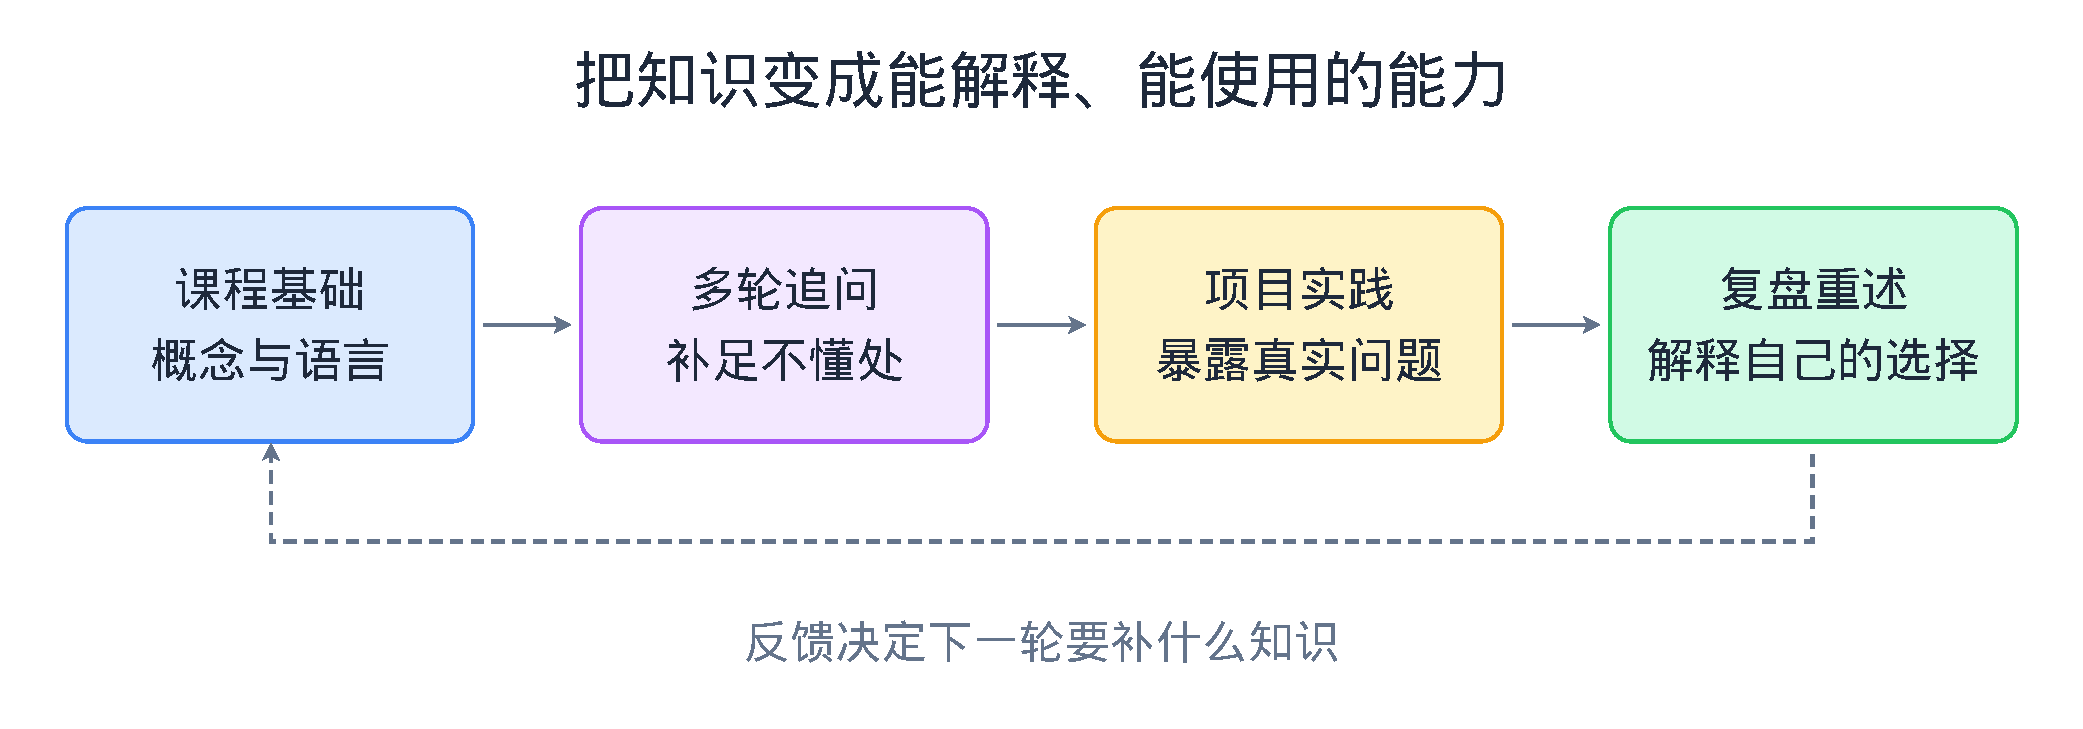
\includegraphics[width=\linewidth,height=.68\textheight,keepaspectratio]{assets/learning-loop.pdf}
\caption{把知识变成能解释、能使用的能力（06:38–12:11，依据节目口述整理的机制示意图）}
\end{figure}
\begin{knowledgebox}{读图：从法律课堂到 AI 项目}
请顺着图中从左至右的实线箭头依次阅读四个横向方框：第一栏是“课程基础：概念与语言”，对应从教材与公开课获取基本认知；第二栏是“多轮追问：补足不懂处”，即针对卡点与模型展开深度问答；第三栏是“项目实践：暴露真实问题”；第四栏是“复盘重述：解释自己的选择”，如在考场手写论述中独立组织论证链。底部的虚线箭头从最右侧回到最左侧，结合底部提示“反馈决定下一轮要补什么知识”，构成了完整的学习闭环。
\end{knowledgebox}
这一闭环说明，AI 的介入之所以没有削弱他对公司法与编程的理解，关键在于末端始终保留了项目实战与复盘重述的硬性检验，用真实反馈指导下一轮该回头补齐哪些基础知识。
\needspace{6\baselineskip}\subsection{本章小结}
本章跟随清华大学法学本科生 Alfred 的视角，展示了如何将初级法律岗位的职业冲击转化为跨学科学习的动力：
\begin{enumerate}
\item \textbf{认知底座不可省}：约 30\% 的教材与公开课学习负责提供学科常识与基础语言，为有效提问打底。
\item \textbf{多轮追问与项目复盘}：约 70\% 的能力提升来自层层深入的 AI 对话，以及在真实项目中边做边学。
\item \textbf{以输出倒逼内化}：通过把课件与教材封装进模型进行模拟出题和观点对话，训练“论点—推理—法理—法条”的论证链，最终在脱离工具的现场手写考试中验证真实掌握度。
\end{enumerate}
\needspace{8\baselineskip}\section{大学的价值如何重新分配}
上一章看到，林桐宇（Alfred）用公开课打底，再靠对话追问和模拟出题掌握了法律与编程基础。当知识获取与代码编写能由工具分担，大学靠统一考卷筛选技能的评估方式开始松动。本章结合 Alfred 与侯泰羽（Kolento）的经历，探讨大学价值如何从单一技能训练转向自我认知、人际信任与价值判断。
\needspace{6\baselineskip}\subsection{职业训练与自我认识}
当学生用工具就能写出漂亮的代码、完成从前依赖死记硬背的作业时，大学原有的考核标准面临直接挑战。Alfred 在清华大学观察到，早期他选修 Python 课程时，老师非常抵触学生用 AI 写代码，一旦认定使用就可能面临学术不端与挂科；学生为了交差，反而要花不少时间故意加入拼写错误（typo）或使用去 AI 痕迹的工具，让代码显得“笨一点”。而到了近两年，计算机系的限制明显放宽，甚至开始在部分考核中鼓励使用 AI，不过他在法学院还没有看到同样明确的转向（12:12–13:42）。

在 Alfred 看来，用旧标准评判学生之所以脱节，是因为训练模型与培养学生面临着相似的困境：许多模型在\textbf{基准测试}（benchmark，用于衡量模型能力的标准化测试集）上得分很高，一旦放进开放环境处理真实任务却表现糟糕；同样，一个擅长应试的高分学生，面对没有标准答案的现实问题也可能束手无策。他认为大学原本同时承载着两层价值，如今第二层正在被工具削弱：

许多名校学生把全部精力放在第二层，直到站上毕业领奖台仍答不出第一层的问题。但对接收、处理并输出信息的知识工作者而言，AI 在常规技能上做得更快、更便宜且全天候在线。为了跳出这种被动局面，Alfred 在北大上过一门类似西方博雅教育的课程后，开始结合个人兴趣调整本科选课策略：主动避开自己不感兴趣、在他看来偏重记忆且与直接就业高度对口的证券法资本市场实务、国际贸易仲裁、贸易法等课程，转而把精力投入更注重训练批判性思考的课程，如法学院的西方法律思想史、法理学、宪法学，以及清华大学新雅书院的西方近代哲学（16:17–17:27）。

许多名校学生把全部精力放在第二层，直到站上毕业领奖台仍答不出第一层的问题。但对接收、处理并输出信息的知识工作者而言，AI 在常规技能上做得更快、更便宜且全天候在线。为了跳出这种被动局面，Alfred 在北大上过一门类似西方博雅教育的课程后，开始刻意调整本科选课策略：避开证券法实务、国际贸易仲裁、贸易法这类偏重记忆与直接就业对口的课程，转而选修法学院的西方法律思想史、法理学、宪法学，以及清华大学新雅书院的西方近代哲学（16:17–17:27）。

在那门西方近代哲学课上，整学期的核心任务就是精读笛卡尔的原著《第一哲学沉思集》。真正读进去之后，Alfred 经历了一段精神上的恍惚：原本习以为常的世界观被拆解了，他开始用批判性的眼光审视周围的一切。当所有的预设都被怀疑和解构时，他并没有滑向虚无主义，反而看清了哪些底层的东西是始终存在的。这次阅读体验让他触碰到很难被 AI 替代的批判性思考，也让他在后续选课、阅读和与世界交互时不再随波逐流，开始从零到一去追问“我是谁、我喜欢什么”（17:27–19:00）。

\needspace{6\baselineskip}\subsection{同辈、导师与信任关系}
既然许多具体的法律实务或初级编程任务都能被工具分担，名校经历留给学生最宝贵的财富是什么？面对主持人的追问，Alfred 首先澄清，他并不认为任何人或任何单一职位是不可替代的；如果总结清华大学带给他的独特财富，他归结为两点：优秀的同侪环境与顶尖的师资力量（20:18–20:51）。

大一刚入学时，Alfred 曾经历过强烈的心理落差。他在高中是全校第一、二名，进入清华后却排到了后 50\%，一度怀疑自己是不是不该来这里。但他很快调整了心态：当五湖四海、不同专业且比自己优秀的同学因为共同兴趣聚在一起，每一次交流都成了向朋友兼老师学习的机会。除了同辈，他还高频利用老师的\textbf{固定答疑与交流时间}（office hour，教授每周预留给学生探讨学业或个人规划的专属时间）进行一对一深聊。他发现，同辈交流重在视野碰撞，而既有学科积累又有社会阅历的导师，能帮他提前看清长远趋势，避开不必要的弯路（21:03–21:49）。

从与同辈和导师的互动中，Alfred 提炼出自己在 AI 时代更看重的一项长处：\textbf{建立人际连接与信任的能力}（people connection）。当外围的技术技能不再稀缺，如何与人建立深度信任并说服他人，直接决定了进入一个新环境后能调动多少资源。主持人由此联想到马斯克近期在访谈中的观点——未来许多大学知识会过时，教育的核心在于培养好奇心、创造力、批判性思维以及社交。Alfred 对此很认同：如果能带着现在的认知回到大一，他会拼命去“社交”，但绝不是去泡吧或赶场参加热闹的活动，而是去争取更多一对一的深度交流（21:50–22:57）。

在纽约大学读应用心理学的 Kolento 则把这种“社交与环境”的思路延伸到了校园之外。他在申请纽约大学的文书里就直接写明“上大学最重要的目的是社交”。最初他曾考虑去多伦多大学，因为深度学习先驱 Geoffrey Hinton 在那里任教，但后来他了解到 Hinton 并不经常教课，便转向了 Hinton 的学生杨立昆（Yann LeCun）任教的纽约大学，并在平时旁听深度学习课程。同时，他长期与硅谷创业者、投资人保持联系，把大量课余时间投入到校外的智能体（Agent，能自主规划并调用工具完成任务的 AI 系统）开发与行业交流中（23:05–24:46）。

\needspace{6\baselineskip}\subsection{学历信号和价值判断}
把大量时间花在校外项目、读论文和行业交流上之后，Kolento 也重新审视了大学课堂与毕业文凭的意义。他回忆，自己在试用 ChatGPT 时对比了早它约 11 年问世的早期语音助手 Siri：早期 Siri 的典型逻辑是先识别用户意图，再匹配到工程师预设好的执行路径；而 GPT 中的 T 代表 \textbf{Transformer}（一种基于自注意力机制的深度学习架构），它的底层逻辑是在概率分布上预测下一个 \textbf{Token}（模型处理文本的基本词元单位）。由于训练数据覆盖了海量的人类文本，它的能力边界不再受限于预设的工程规则，几乎什么话都能接。这种开放解答能力让 Kolento 觉得，与其按部就班地听取为标准化教育设计的预设课程，不如把更多时间花在与 AI 共处、看论文和做自己的产品上（24:48–26:07）。

尽管上课常常在看自己的论文，Kolento 却坦言自己上大学的目的非常务实——就是为了拿一个学历。他不认同“AI 时代学历会消失”的说法，并认为网络上关于“技能可替代所以学历贬值”与“学历代表人的质量所以不贬值”的争论，都只看到了一部分表象。在他的分析中，要看清背后的结构性逻辑，需要把学历视为一种向市场传递“这个人可以被信任、可以委以重任”的社会信号，而不仅仅是对个人所学知识的证明。他认为少数跳过大学依然成功的案例存在\textbf{幸存者偏差}（survivorship bias，因只看到成功样本而忽略庞大失败基数的认知偏差）；从古代苏美尔人的泥板学校到近代工业学校，教育制度之所以能长久留存，在他的理解里始终与人才筛选和评估高度相关。在未来高度不确定的情况下，拿到这张社会信任凭证对他而言依然重要（26:29–28:34）。

除了获取外部凭证，Kolento 将自己在大学里最想习得的核心能力概括为“评估”。在他看来，当大量的执行类流程被 AI 切走后，留给人的关键工作就是做价值判断。这种思考让他着迷于西方哲学对\textbf{美德}（Virtue）与“好”的追问。他认为，面对技术乐观主义，人更需要居安思危；文科与通识教育的意义在于培养人的美德、让人分辨什么是好与坏，从而驾驭技术，而非停留在单纯的计算上。虽然像柏拉图所说的理念世界那样，“好”与“美德”是抽象的极致概念，人很难给出标准定义，但“虽不能至，心向往之”，持续追问这些概念正是人确立价值标准的过程（28:47–29:54）。

落回日常的专业课学习，Kolento 选择用尽可能少的时间掌握应用心理学的核心内容，把腾出来的精力全部投入到与 AI 对话、探索哲学以及做创业产品和实习中。他很推崇斯坦福大学教授在《设计你的人生》（Design Your Life）一书中提出的理念：不要为中长期目标做僵化的强预设，而要在短期内通过高密度的尝试与试错，在实际反馈中摸清自己真正想要什么。虽然 Alfred 是从法学与哲学阅读中向内确立自我认知，Kolento 是把文凭当作信任底牌、向外做高频产品试错，但两人都把大学从“技能培训所”改造成了探索自我与锤炼判断力的试验场（29:59–31:07）。

\begin{importantbox}{区分大学的双层价值与个人发力点}
Alfred 将大学教育拆解为两个维度：
\begin{itemize}
\item \textbf{社会工具价值}：掌握特定学科的知识壁垒与实务技能，直接服务于求职谋生。
\item \textbf{自我认知价值}：通过博雅教育、哲学阅读与批判性思考，弄清个人热情、能力边界与人生方向。
\end{itemize}
当常规的信息处理与代码编写被工具分担时，单纯依赖第一层容易陷入被动，主动补齐第二层才能建立长期的判断支点。
\end{importantbox}
\begin{knowledgebox}{为什么说“学历是一种社会信任信号”}
在 Kolento 的分析框架中，教育的社会功能与个人学习体验是分开的：
\begin{itemize}
\item \textbf{对内（个人能力）}：通过项目实践与通识思考训练“评估”能力，即在AI生成的众多结果中做价值判断。
\item \textbf{对外（社会信号）}：市场在筛选人才时面临高昂的信息核实成本，文凭充当了降低信任成本的标准化凭证。因此，即便具体课程内容可以通过个性化工具自学，学位的筛选与背书机制在短期内依然有效。
\end{itemize}
\end{knowledgebox}
\begin{table}[H]\centering\small
\caption{AI 冲击下大学核心要素的价值重估}
\begin{tabular}{>{\raggedright\arraybackslash}p{\dimexpr(\linewidth-6\tabcolsep)/3\relax}>{\raggedright\arraybackslash}p{\dimexpr(\linewidth-6\tabcolsep)/3\relax}>{\raggedright\arraybackslash}p{\dimexpr(\linewidth-6\tabcolsep)/3\relax}}
\toprule
大学传统要素 & 面临的现实冲击 & 访谈嘉宾的应对与重构\\\midrule
实务与记忆型课程 & 条款分析、文书与基础代码可由 AI 快速生成 & 避开纯记忆课，选修思想史与哲学原著以训练批判性思维\\[4pt]
标准化作业与考试 & 高分学生或高分模型在开放真实环境中可能表现糟糕 & 减少在预设标准课上的消耗，把精力转向真实项目与试错\\[4pt]
同辈与导师资源 & 单靠课堂听讲难以获得针对个人困境的反馈 & 利用 office hour 与导师深聊，与跨专业同辈建立一对一深度连接\\[4pt]
毕业文凭与学位 & 知识获取门槛降低引发“学历贬值或消失”的争论 & 将学历视为面向市场的社会信任凭证，同时在校内外锤炼评估能力\\[4pt]
\bottomrule\end{tabular}\end{table}
当常规的信息检索、文书起草与基础代码编写越来越容易被工具分担，名校学生该如何重新安放大学四年的精力？结合林桐宇（Alfred）与侯泰羽（Kolento）在访谈中的探讨，下图将大学所能提供的资源拆解为四个并列维度。
\begin{figure}[H]\centering
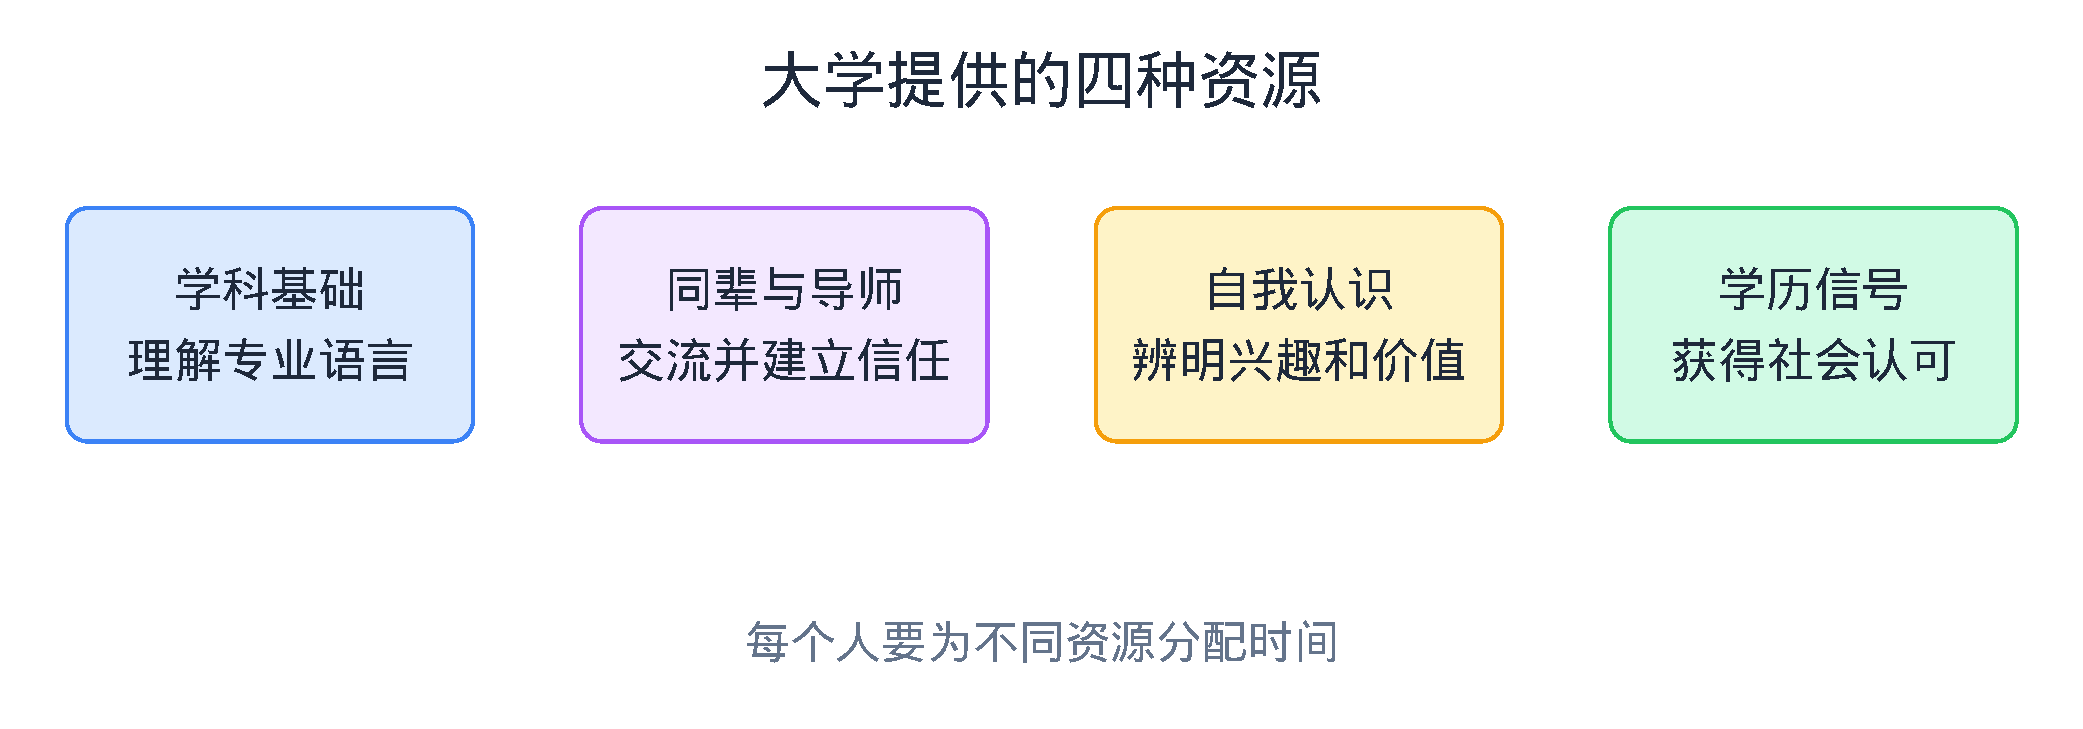
\includegraphics[width=\linewidth,height=.68\textheight,keepaspectratio]{assets/university-value.pdf}
\caption{大学提供的四种资源（14:43–31:07，依据节目口述整理的机制示意图）}
\end{figure}
\begin{knowledgebox}{读图：大学的价值如何重新分配}
图中采用无箭头的四栏横向并列结构，依次列出大学提供的四类资源：第一栏是“学科基础：理解专业语言”；第二栏是“同辈与导师：交流并建立信任”，如 Alfred 利用 office hour 与教授深聊、向优秀同辈学习；第三栏是“自我认识：辨明兴趣和价值”，对应他精读哲学原著后的自我追问；第四栏是“学历信号：获得社会认可”，即 Kolento 所看重的面向市场的信任凭证。图底标注提醒“每个人要为不同资源分配时间”。
\end{knowledgebox}
两位嘉宾虽然对这四栏资源分配了不同权重——Alfred 重视师生深度连接与向内探索自我，Kolento 则以学历信号为底牌向外做高频产品试错，但两人都跳出了单一的应试技能竞争，主动重构了各自大学生活的重心。
\needspace{6\baselineskip}\subsection{本章小结}
本章梳理了两位名校生对大学价值的重新分配：
\begin{enumerate}
\item \textbf{从技能训练转向自我认知}：Alfred 通过选修思想史与精读《第一哲学沉思集》，在职业技能被工具冲击时确立批判性思考与自我定位。
\item \textbf{从泛化社交转向深度信任}：善用同辈切磋与导师 office hour，把核心竞争力锚定在建立人际信任与深度沟通上。
\item \textbf{分清外部凭证与内部判断}：Kolento 将学历视为降低市场交易成本的信任信号，同时用短期高频的产品与实习试错来训练价值判断力。
\end{enumerate}
\needspace{8\baselineskip}\section{个性化学习如何走到理解}
上一章讨论了大学在自我认识、人际关系与学历信号上的价值重新分配。但回到具体的学习过程：当课堂要求和工具环境发生剧烈分化，学生如何利用 AI 真正学会一门知识，而不是停留在表面答案？本章将沿着教师评价的转向、理解速度与深度的争论，拆解如何从优秀作品出发反推个人学习路径。
\needspace{6\baselineskip}\subsection{教师的分歧与评价方式}
围绕判断力的培养，大学教师在日常教学中对 AI 工具的态度正呈现出明显分化。侯泰羽（Kolento）观察到，即使在同一所学校里，不同课程的要求也截然不同（31:46–32:31）。在他主修的应用心理学必修论文课上，老师直到毕业前的最后一节课，还在给全班发放印有“不要使用 GPT”的贴纸；而在另一门教授网站制作全流程的选修课上，老师在开学第一天就让学生放下传统编程软件，直接上手 \textbf{Claude Code}（命令行编程代理工具）、\textbf{Replit}（在线协同编程与部署平台）和 \textbf{Lovable}（通过自然语言构建全栈应用的工具）。这种强烈反差让他感到，教学与其一味限制工具，不如教学生跟进最新工具，并在工具不断演进的环境中建立自己的判断力。

为了说明为什么持续的竞争力来自价值判断而非单纯使用工具的熟练度，Kolento 转述了麻省理工学院计算机科学教授、早期对话程序 \textbf{ELIZA} 的作者 \textbf{Joseph Weizenbaum} 的观点，用来讨论两类不同的过程（32:41–33:45）：

\begin{enumerate}
\item \textbf{决策（deciding）}：Kolento 将其解释为在给定条件后按规则推导、存在标准答案的推理过程，他在举例时提到了下棋、诊断部分疾病或计算最短路径，认为这类按规则推导的任务适合交给机器执行。
\item \textbf{选择（choosing）}：指在缺乏客观标准时依然需要做出的取舍与判断，它根植于人的经历、价值观以及对他人痛苦的感受能力。Kolento 举了法官判刑的例子：即使向机器输入所有案件事实，最终关乎生死与是否坐牢的决定依然要交给人来承担（注：现实中的医疗诊断与司法裁判同样包含复杂的价值权衡与伦理责任，此处为嘉宾借用该框架说明规则推导与价值取舍的区别）。
\end{enumerate}

在 Kolento 看来，这种判断能力与“如何学习”一样，属于跨越时代的\textbf{元能力（meta-skill）}。当外层的工具包装持续演进时，高校的考核方式也可能会随之调整（33:49–34:36）。他结合自己在纽约大学看到的成立主打 AI 专业的新学院等动向，以及斯坦福大学将传统编程课改为 \textbf{Vibe Coding}（主要通过自然语言提示词与 AI 协作生成代码的开发方式）课程的观察，提出了一个猜想：从 2026 年开始，随着更多老师提倡用 AI 解决问题，考试形式可能会从传统笔试转向口试，而学生的创作空间也会部分从纸面文章转移到对话框中——即如何构建高质量的 \textbf{Prompt}（提示词，输入给模型的指令与上下文）来引导生成过程。

\needspace{6\baselineskip}\subsection{理解速度争论的两个层次}
随着交互重心转向与模型对话，AI 究竟能否加快人的理解过程？围绕这个问题，主播泓君与 Kolento 展开了一段直接的交锋（34:37–36:28）。泓君首先提出，从她自己的感受来看，AI 虽然能放大能力、帮人快速完成任务或给出许多答案，但并不会加速理解过程本身。她以花同样时间完整阅读一篇学术论文或踏实消化一份应用心理学课件为例指出，人脑在单位时间内吸收和消化深层原理的处理速度与容量是有限的；当问题已经非常明确、需要把一个特定问题彻底弄懂时，AI 只能提供更好的资料，却很难替大脑省去那个必须亲自学习的单位时间。

Kolento 则从信息获取的维度提出了相反的看法（35:10–35:31）。他认为在信息过载的环境下，人的认知带宽有限，而 AI 可以根据学习者当前的知识背景与上下文，筛选出先看什么、后看什么，指出哪些材料对当前问题最有帮助。从减少无效检索、精准匹配学习材料的角度来看，AI 确实在辅助加速整个理解进程。

两人的争论提示我们，可以把学习过程拆分为两个不同层面来观察（35:32–36:36）：
\begin{itemize}
\item \textbf{信息筛选的广度与材料匹配}：在面对海量信息时，依靠 AI 过滤噪音、按个人当前上下文定制阅读优先级，能够减少无效摸索，从宽度和路径匹配上辅助推进学习。
\item \textbf{特定问题的深度消化}：当学习者已经锁定了一个具体问题（如消化专业课件原理、理解哲学与法律历史的由来或推进前沿科学研究），泓君强调依然需要靠人脑投入单位时间去扎实咀嚼；这种理解的深度，反过来又会影响一个人能把 AI 工具用到多深。
\end{itemize}

\needspace{6\baselineskip}\subsection{从好作品反推自己的学习路径}
基于上述关于信息筛选与深度理解的讨论，Kolento 分享了他自己使用 AI 的\textbf{逆向学习法（top-down，自顶向下）}，用来对比传统教育常见的\textbf{自底向上（bottom-up）}路径（36:37–37:58）。在他看来，传统路径要求学生先花大量时间打基础，但很多人走到一半容易迷失方向，不清楚为什么要打这些基础，也不知道最终要走到哪里。而在 AI 能够直接给出参考答案或指向高水平解读的条件下，学习者可以先看见一个真实的锚点：先了解最顶尖的人怎么思考、接触顶级作品，训练自己感知好坏差异的评估标准；当鉴赏能力走在生产能力前面时，对自身产出的不满意就会驱使自己持续深度学习与迭代。

为了让这种自顶向下的学习不被顶层的庞大信息量压垮，Kolento 强调他给自己的心智原则是“找关键区分点，而不是学全部”。他以自己学习 \textbf{Transformer} 原理的经历说明具体做法（37:58–39:19）：传统路径通常要先学数学、线性代数（Linear Algebra）和机器学习（Machine Learning）；而他在学习时，先通过 Prompt 让 AI 模拟一个由 Geoffrey Hinton、Yann LeCun 等人组成的“专家团”，帮他梳理出 Transformer 的原理框架，再直接针对里面没听懂的具体概念，让 AI 给出定义和实例。

需要明确的是，大语言模型组织的“专家团”只是提示词激发出的模拟视角，并非真实学者的发言，模型给出的答案也未必准确。为了判断答案对错，Kolento 在追问过程中会固定做两步校验处理（38:36–39:19）：
\begin{enumerate}
\item \textbf{联网查证原始出处}：要求 AI 开启上网搜索，给出可以点击验证的链接（Link），或者自己上网核查。
\item \textbf{向身边的真人请教}：去问身边真正精通该领域的朋友，把真人专家的确认反馈作为“可验证的奖励”，借此判断自己的理解是否正确、能否继续往前推进。
\end{enumerate}
在 Kolento 看来，正向路径是教材设计者预设的通用路线，而这种“先确立顶层锚点—顺着个人不懂的卡点追问关键区分点—用网页链接与真人反馈验证”的逆向路径，是他为了更快抵达具体学习目标而采取的个性化路径。

\begin{knowledgebox}{理解“专家团提示词”与双通道验证机制}
在逆向学习中，让 AI 扮演顶尖学者（如“专家团”）是一种激发高质量解释框架的提示技巧，目的是快速调出该领域的核心概念图谱，但它并不代表真实学者的观点。要将模型输出转化为可靠理解，必须配合双通道验证：
\begin{itemize}
\item \textbf{文献通道}：强制要求模型提供外部网页或论文链接，核查原始定义。
\item \textbf{人际通道}：向领域内的真人专家复述理解，获取纠偏反馈。
\end{itemize}
\end{knowledgebox}
\begin{importantbox}{区分学习中的“信息检索”与“认知内化”}
泓君与 Kolento 的讨论提示我们区分学习中的两个环节：第一个环节是\textbf{找路与选材}，AI 能根据个人背景过滤无关信息，缩短定位相关概念的时间；第二个环节是\textbf{深度消化}，即花时间把具体课件、论文或历史渊源吃透，这一过程依然需要学习者亲自投入时间与精力，而理解的深度又会反过来影响后续使用 AI 的深度。
\end{importantbox}
\begin{table}[H]\centering\small
\caption{正向基础路径与逆向锚点路径对照}
\begin{tabular}{>{\raggedright\arraybackslash}p{\dimexpr(\linewidth-6\tabcolsep)/3\relax}>{\raggedright\arraybackslash}p{\dimexpr(\linewidth-6\tabcolsep)/3\relax}>{\raggedright\arraybackslash}p{\dimexpr(\linewidth-6\tabcolsep)/3\relax}}
\toprule
比较维度 & 正向路径（自底向上） & 逆向路径（自顶向下）\\\midrule
起点设定 & 按教材大纲先学前置数学与基础理论 & 先接触优秀作品与顶层原理框架，建立鉴赏锚点\\[4pt]
推进逻辑 & 沿标准化课程预设的顺序逐步推导 & 顺着个人理解卡点追问，只抓关键区分点\\[4pt]
常见风险 & 战线过长，容易在中途丧失目标感与动力 & 被顶层信息量压垮，或误信模型生成的错误解释\\[4pt]
校准方式 & 依靠课后习题与阶段性标准考试 & 要求模型提供可查证链接，并向懂行的真人请教确认\\[4pt]
\bottomrule\end{tabular}\end{table}
传统教材往往要求学生按部就班地从前置数学和基础概念学起，容易让人在中途丧失目标感。侯泰羽（Kolento）结合自己跨界学习深度学习架构的经历，提出了一套自顶向下的逆向学习流程，其推进步骤如下图所示。
\begin{figure}[H]\centering
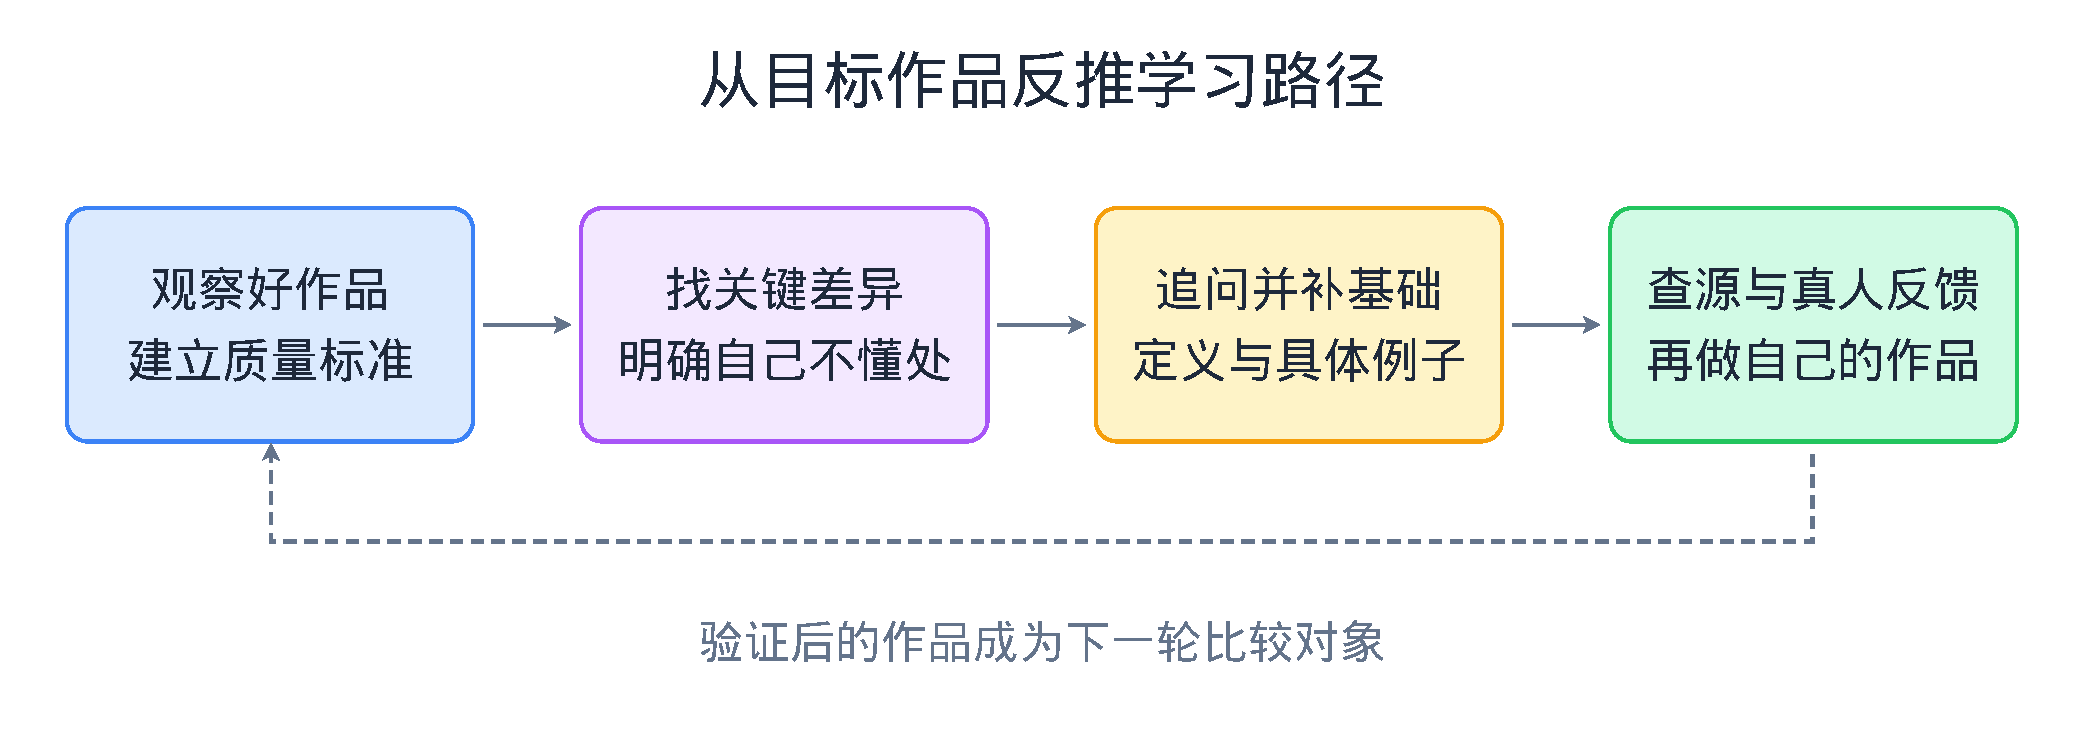
\includegraphics[width=\linewidth,height=.68\textheight,keepaspectratio]{assets/reverse-learning.pdf}
\caption{从目标作品反推学习路径（36:26–39:19，依据节目口述整理的机制示意图）}
\end{figure}
\begin{knowledgebox}{读图：个性化学习如何走到理解}
顺着图中从左到右的实线箭头，四个横向方框依次为：第一栏“观察好作品：建立质量标准”，先接触高水平产出以确立鉴赏锚点；第二栏“找关键差异：明确自己不懂处”，不求一次学完所有前置科目，而是定位阻碍理解的核心卡点；第三栏“追问并补基础：定义与具体例子”，让模型针对卡点给出清晰解释与实例；第四栏“查源与真人反馈：再做自己的作品”。底部虚线箭头从最右端回指最左端，表明“验证后的作品成为下一轮比较对象”。
\end{knowledgebox}
这四个环节提醒我们，提示词模拟出的“专家团”只是打开思路的启发工具；唯有在末端落实联网查证出处与请教真人专家，并在做出自己的作品后开启下一轮比较，按需倒推的个性化路径才能真正走向扎实理解。
\needspace{6\baselineskip}\subsection{本章小结}
本章围绕个性化学习如何走向真正理解展开：
\begin{enumerate}
\item 课堂对 AI 的态度正发生分化，超越工具本身的持久竞争力在于做价值取舍的“选择（choosing）”与评估能力。
\item AI 能在广度上通过信息筛选加速学习路径匹配，但人脑对特定问题深层原理的消化仍需投入必要的单位时间。
\item 逆向学习通过先看优秀标杆、追问个人卡点，并结合外部链接核查与真人反馈，构建出贴合个人需求的个性化理解闭环。
\end{enumerate}
\needspace{8\baselineskip}\section{让 AI 参与作业，也保留自己的判断}
在上一章中，Kolento分享了利用AI模拟视角并进行逆向学习的个人路径。进入具体的日常学业，当AI能够处理绝大多数课业环节时，学生究竟是在把作业交给机器代笔，还是在重构做题流程？本章通过纽约大学数据科学本科、哥伦比亚大学管理科学与工程硕士饶杰武（Jack）的经历，探讨如何在高频使用AI参与作业的同时，拆解需求并守住个人的判断力。
\needspace{6\baselineskip}\subsection{99\% 参与意味着什么}
顺着个性化学习的讨论，话题自然延伸到了日常课业中 AI 的实际介入程度。与大一就遇上 ChatGPT 的 Alfred 和 Kolento 不同，饶杰武（Jack）于 2020 年入学，并在进入大学前就接触过编程。他在 2022 年底大三时帮纽约大学教授做科研项目，当时他主修的数据科学（Data Science）课程并没有教授计算机科学（CS）中的前端开发，而项目恰好需要做出一个前端网站。于是他借助刚上线的 ChatGPT 把网站搭建了出来，随后又在日常中陆续用起 Claude、Perplexity（结合实时网页检索的问答工具），以及专门辅助写代码的编程智能体（Coding Agent）和 Manus、Genspark 等通用代理工具（39:19–40:28）。

当被主持人泓君问到有多少作业或论文是由 AI 帮忙写的时候，Jack 先脱口而出“99\%”，紧接着在追问下做了关键的语义纠正：并不是指作业由 AI 代写，而是指在 99\% 的作业中，AI 都在里面占了很大的参与比例。至于剩下的 1\%，他举了录制口头展示（Presentation）视频的例子——这类环节目前仍必须由他本人开口去讲；而就作业本体而言，他已经想不到有哪些作业完全没有 AI 的参与了。这种重度参与从 2022 年底至 2023 年初延续下来，面对任何新的作业或课题，他的第一步通常是先问问 AI 的想法（40:51–41:48）。

面对学生高频使用 AI 的现状，Jack 观察到学校教授的态度也经历了从早期非常抵触到最近一两个学期逐步接受的转变。虽然大学里一直配有 Turnitin（高校常用的学术论文原创性比对与 AI 生成文本检测系统）这类监测软件，但他认为监测工具并不会让学生彻底远离 AI，而是促使人与 AI 更好地协作完成任务。越来越常见的课堂共识是：学生可以向大语言模型（LLM，Large Language Model，基于海量文本训练、擅长生成与处理自然语言的 AI 模型）咨询，但学生本人必须对最终提交的产出负责（41:48–42:42）。

\needspace{6\baselineskip}\subsection{先拆需求，再检查候选答案}
在同学普遍使用 AI 的情况下，交上去的作业与论文依然有好坏之分。Jack 将日常作业区分为两类来说明判断标准（42:43–43:14）：
\begin{itemize}
\item \textbf{可验证的作业}：例如数学题，存在明确的标准答案，对错可以直接验证。
\item \textbf{非可直接验证的开放性作业}：例如撰写论文或开发一个网站，教授批改时通常不直接判对错，而是评估作品整体做得较好还是较差。
\end{itemize}

在应对开放性作业时，Jack 会先拿模型做“需求拆解”。他把课程背景和作业要求输入给 AI，询问应该从哪些角度思考这个问题，借此理清第一件事、第二件事分别要做什么。接下去的操作则取决于他对课程的熟悉程度：如果是机器学习（Machine Learning）这类他比较熟悉的课程，需要写前置代码时，他会很自然地自己打开 Google Colab（谷歌提供的云端交互式代码运行环境），手动切换运行时（Runtime）并做好基础设定；如果遇到自己不太了解的课程，他才会更大程度地依赖 AI 去把这些前序准备工作做得更好一些（43:15–43:53）。

在需求拆解和生成内容之后，作业成绩的高低取决于学生的课程理解深度与价值判断能力。Jack 举例说，如果一个学生压根没学这门课，不知道 AI 写出来的内容是对是错就直接交上去，那大概率不会是一份好产出；相反，如果学生既会用 AI 工具，又对课程本身很了解，能判断出 AI 产出的内容是否可用，并在修改、去掉生硬的“AI 味”且通过最终检测后提交，在他的经验里这类作业往往能拿到 80 分、90 分甚至更高。泓君也补充道，只有对课程理解得深，才能识破 AI 是否在“胡说八道”。尤其在做网站等开放任务时，Jack 指出 AI 一次可以给出三个甚至十个方案，如果你反问 AI 挑哪一个，它往往会说每一个都是好方案，因此最终的价值判断与取舍依然会落回人身上（44:11–45:34）。

\needspace{6\baselineskip}\subsection{把省下的时间用到推理上}
当 AI 接管了大量前序准备与资料查找工作后，Jack 表示留给自己学习和思考的时间反而更多了。为了说明这一点，他对比了使用 AI 前后的查找过程：以前在思考过程中遇到问题，往往需要自己翻书或上网搜索，许多信息藏在互联网深处，可能要花很长一段时间才能找到正确答案（43:55–46:01）。

在Jack看来，这种纯粹为了翻找现成资料而耗费时间的过程，并没有真正把他变成一个更好的学生，只是在单纯消耗精力。引入AI之后，原本散落的信息可以被快速索取和汇总，且准确度比早期更高。这相当于用工具切掉了那些机械、无关紧要的检索步骤，把原本被检索占用的时间释放了出来（43:55–46:11）。

这样一来，个人精力的分配发生了转移：以前耗在机械搜索上的时间被省了下来，现在可以用来与 AI 交流思考、做头脑风暴（脑暴），并消化课程的核心逻辑。通过压缩低价值的翻找步骤，学习者有条件把更多时间投入到真正影响作业质量的推理、验证与判断上（46:08–46:18）。

\begin{warningbox}{区分“AI参与率”与“AI代写率”}
访谈中提到的“99\%”极易被误解为“99\%的作业直接由AI生成后原样交差”。Jack在对话中专门纠正了这一说法：
\begin{itemize}
\item \textbf{AI参与}：将AI用于启发角度、拆解任务要求、生成候选方案以及快速检索资料，人依然主导配置与筛选。
\item \textbf{AI代写}：不经学习与核验，直接将模型输出作为最终结果提交。把高参与度等同于纯代写，会掩盖人在需求拆解与质量把关上的核心工作。
\end{itemize}
\end{warningbox}
\begin{knowledgebox}{为什么开放性作业无法连同“选择”一起外包}
在写网站或写论文等非直接验证任务中，大语言模型擅长根据提示词发散出多个看似通顺的候选方案（如3到10个网页设计稿）。但由于缺乏具体课程语境下的真实偏好与责任边界，当你让模型自己挑一个最佳方案时，它往往倾向于肯定每一个选项。只有理解课程核心标准的人，才能完成从“多个候选”到“最终交付”的收敛。
\end{knowledgebox}
\begin{table}[H]\centering\small
\caption{不同课业场景下的AI协作与人工把关对照}
\begin{tabular}{>{\raggedright\arraybackslash}p{\dimexpr(\linewidth-6\tabcolsep)/3\relax}>{\raggedright\arraybackslash}p{\dimexpr(\linewidth-6\tabcolsep)/3\relax}>{\raggedright\arraybackslash}p{\dimexpr(\linewidth-6\tabcolsep)/3\relax}}
\toprule
作业或任务场景 & AI承担的角色 & 人工保留的核心动作\\\midrule
陌生课程的开放作业 & 结合课程要求拆解思考角度，辅助前序准备 & 理清任务的第一、二步顺序，核对内容是否偏题\\[4pt]
熟悉课程（如机器学习） & 提供代码片段参考或特定问题解答 & 自行打开Google Colab配置环境，主导代码结构\\[4pt]
网站开发与多方案设计 & 一次生成3至10个候选方案供挑选 & 依据课程理解评估优劣，拍板做出最终选择\\[4pt]
日常资料与答案查找 & 快速检索并汇总隐藏在网络深处的信息 & 省下机械翻找时间，用于头脑风暴与深度推理\\[4pt]
\bottomrule\end{tabular}\end{table}
饶杰武（Jack）在访谈中提到自己 99\% 的作业都有 AI 参与，但专门纠正这绝非由机器全盘代写。为了厘清高比例参与和人工负责如何在同一套做题过程中并存，下图按先后顺序梳理了他在处理课业时的四个核心环节。
\begin{figure}[H]\centering
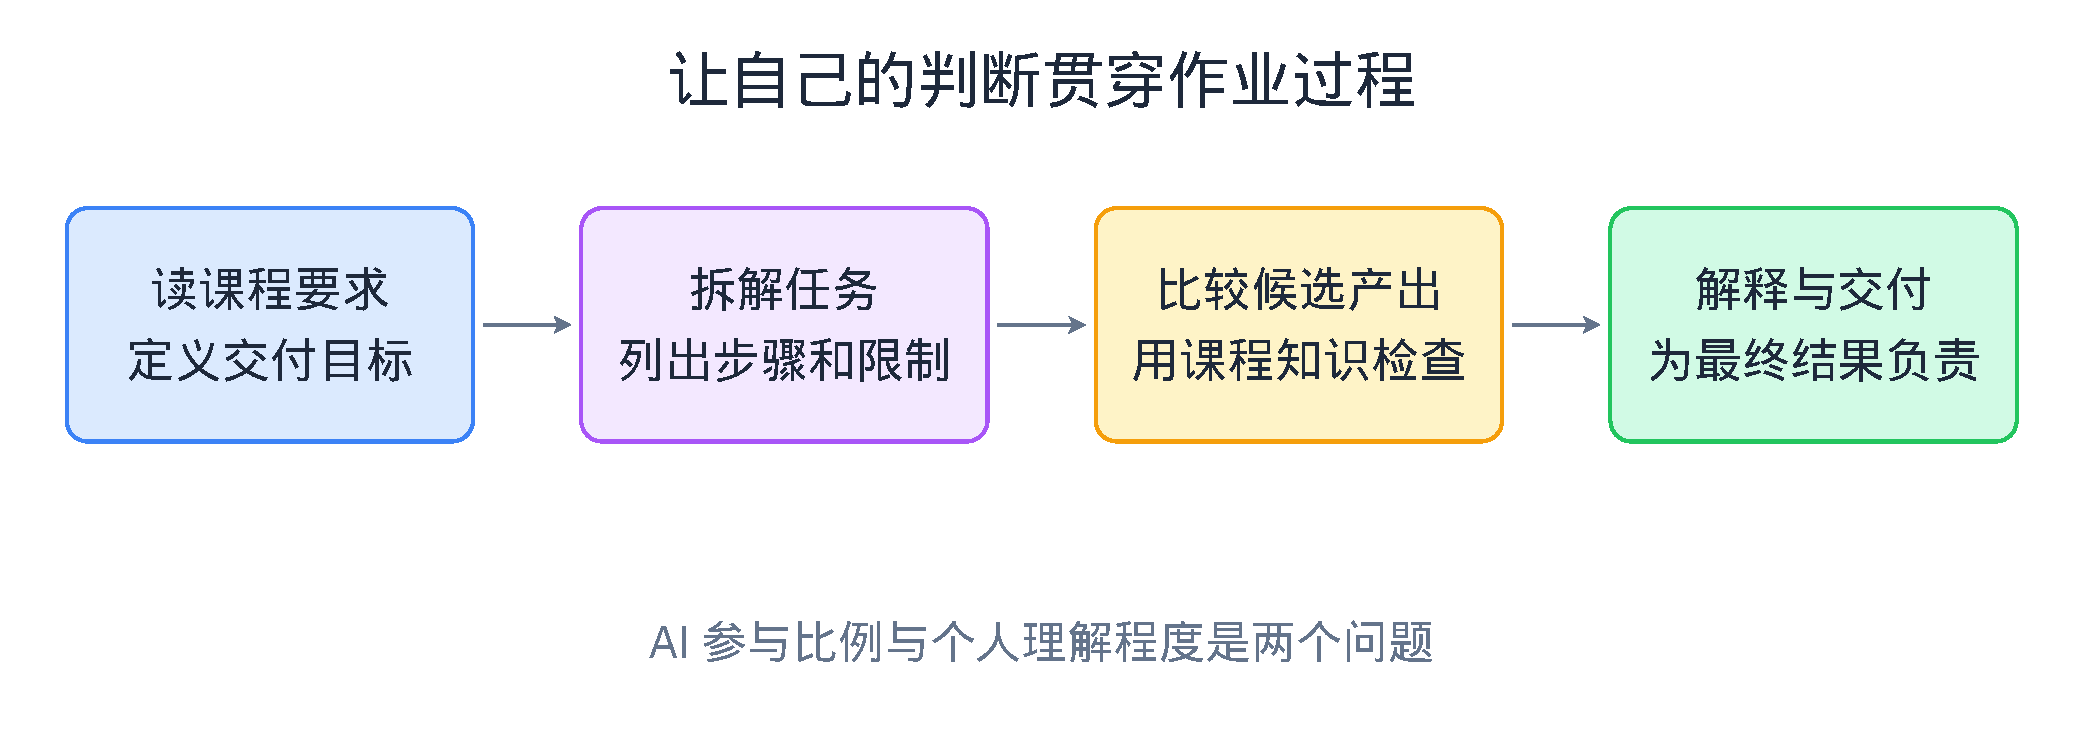
\includegraphics[width=\linewidth,height=.68\textheight,keepaspectratio]{assets/assignment-flow.pdf}
\caption{让自己的判断贯穿作业过程（40:51–46:38，依据节目口述整理的机制示意图）}
\end{figure}
\begin{knowledgebox}{读图：让 AI 参与作业，也保留自己的判断}
图中由左至右以单链实线箭头连接四个方框：第一步是“读课程要求：定义交付目标”，先结合课程背景明确任务方向；第二步是“拆解任务：列出步骤和限制”，理清第一件事、第二件事分别做什么；第三步是“比较候选产出：用课程知识检查”，无论面对有标准答案的习题还是模型生成的多个网页、论文方案，都需靠课程理解辨别优劣；第四步是“解释与交付：为最终结果负责”。图底文字强调“AI 参与比例与个人理解程度是两个问题”。
\end{knowledgebox}
这条单向递进的链条表明，工具省去的是翻书和大海捞针式的机械检索时间；而在比较候选方案与最终交付上，学习者对课程本身的掌握深度依然决定着作业的真实成色。
\needspace{6\baselineskip}\subsection{本章小结}
本章围绕Jack的课业实践，梳理了AI高频参与作业时的完整工作流：
\begin{enumerate}
\item \textbf{明确参与边界}：“99\%参与”是指AI贯穿了从构思到检索的各环节，而非替代本人思考与表达，学生仍需对产出负责。
\item \textbf{分层处理任务}：先让AI协助拆解作业要求，再根据自身对课程的熟悉度调整介入深度；在开放任务的多方案对比中，依赖扎实的课程理解做出最终取舍。
\item \textbf{重构时间分配}：用AI压缩翻书和大海捞针式的机械检索时间，将省下的精力转移到头脑风暴与核心推理上。
\end{enumerate}
\needspace{8\baselineskip}\section{从工具清单到个人工作流}
上一章讨论了如何在作业中拆解需求并验证候选答案。当 AI 工具从单一对话框扩展到语音输入、图形生成与多步代理时，新的问题随之出现：面对层出不穷的产品，学习者和开发者该如何避免盲目收集工具，转而按自己的任务链路组合出清晰、可控且成本合理的个人工作流？
\needspace{6\baselineskip}\subsection{把输入、探索与执行分开}
除了在课业中拆解需求，日常高频使用 AI 的另一个变化是如何组合不同特长的工具。到了 2026 年初节目录制时，三位嘉宾都已经不再把所有需求塞进同一个聊天框，而是根据输入转换、架构探索和具体执行等不同阶段，将工具拆解到各自对应的环节中（46:38–49:32）。

以饶杰武（Jack）的日常开发为例，他在进行 \textbf{Vibe Coding} 时，常常无法在第一时间像写精准提示词那样把需求完整写下来，口头表达往往支支吾吾。为此，他在输入端引入了支持手机与电脑端的语音输入工具 Typeless：先把脑中大概想要的东西说出来，由该工具剔除冗余口水词、挑出重点并转化为规整的书面形式，再传入 Prompt 交给 Claude 或 OpenAI 的 Codex 等 \textbf{Coding Agent}。林桐宇（Alfred）同样在微信长信息回复、写 Prompt 和回邮件时高频使用这一把非结构化语音转为结构化文本（unstructured to structured）的桥梁，并配合桌面快捷启动工具 Raycast 提升调用效率（47:06–49:08）。

除了输入与代码执行，前端视觉探索和论文验证也需要独立的工具角色。Jack 在做动画设计时会先用 Variant 生成多个前端动画方案，挑中后再直接提取代码沿用；在读论文遇到复杂系统架构时，则会用开源大模型应用与工作流编排平台 Dify 搭建实验流来测试想法（46:53–47:55）。Alfred 则将自己的工具箱明确切分为三大类：
\begin{itemize}
\item \textbf{聊天机器人（Chatbot）}：日常高频使用 Gemini 网页端进行基础问答；
\item \textbf{提效入口层}：用 Typeless 和 Raycast 处理语音结构化与快捷调用；
\item \textbf{长程代理（Long-horizon Agent）}：指能够跨越多个步骤、在较长时间窗口内持续自主规划并执行复杂任务的智能体，如 OpenClaw、Manus 与 Claude Code。
\end{itemize}

侯泰羽（Kolento）则分享了他在协同办公与垂直创作上的个人体验（50:11–52:04）。在当时的日常使用中，他个人非常推崇协同工具 Claude Cowork；而在特定创作场景下则选用专项工具：例如在节目录制前两天，他用音乐生成工具 Suno（当时测试的 V5 preview 版本）为自己创业项目的落地页（Landing Page）制作主题曲，并观察到该版本对不同音乐风格提示词的识别比早期版本更准，且在他上传一些小众的他人原创歌曲时能识别出已有作品；在前端视觉上，他使用过 Gemini 的 Dynamic View 功能通过提示词直接生成动态交互界面（生成式 UI）；此外，他还测试了刚上线不久、由 Inception Labs 发布的 Mercury 2，该产品采用 \textbf{Diffusion LM}（扩散语言模型，利用迭代去噪机制并行更新多个位置的文本、区别于传统逐词自回归预测的架构），在他当时的体验中给出提示词后约 3 秒内就能跑出一个前端界面草稿。可见，把口述整理、视觉或架构探索与最终的代码生成拆开，能让每个环节都对应到合适的工具角色。

\needspace{6\baselineskip}\subsection{通用调度和专用工具如何配合}
随着手头的专用代理增多，通用型代理与垂直代理该如何配合？围绕 OpenClaw 出现后是否还需要 Manus 或 Genspark 这类封装好的代理产品，三位嘉宾结合各自的使用习惯给出了不同的选择（52:05–53:55）。

Alfred 的做法是把 OpenClaw 当作日常高频生活事务的入口，同时让它充当 \textbf{Agent Orchestration Layer}（代理编排层，负责理解总任务并在后台调度其他专用代理协同工作的中间层）。在他看来，OpenClaw 单独执行特定垂直任务时的交付质量和效率，尚不及已经打磨成熟的专用代理产品；但它在即时通讯（IM）视窗中的交互及时性，以及跨任务的上下文记忆能力，使它非常适合作为“总管”去调用 Manus（负责深度调研与设计）和 Claude Code（负责软件开发）。因此，引入 OpenClaw 后，他调用其他专用代理的频率反而更高了（49:08–49:32，52:44–53:18）。

在需要深入网页交互的调研场景中，专用工具的封装优势让 Jack 与 Alfred 继续高频使用它们。当想研究某个网站优秀的交互设计，或收集某款产品在 Reddit 与 X（原 Twitter）上的用户评价时，他们会调用具备 \textbf{Browser Use}（浏览器操作能力，即代理在图形界面中直接打开并操作浏览器）的 Manus。Jack 觉得这类产品把复杂技术打包成了对用户友好的形式，省去了自己配置的麻烦；Alfred 则补充说，单纯通过简单的 \textbf{Search API}（搜索应用程序接口）往往拿不到需要操作图形界面（GUI）的深层信息，而在他当时的个人体验中，Manus 可以打开他本地浏览器的标签页、登录账号去浏览对应社区并汇总成一份 \textbf{Deep Research}（深度研究）报告，或在其推出的 Canvas 画布工具中调用 Nano Banana 等图像能力完成设计工作（52:21–52:43，56:30–57:46）。

然而，面对同一个 OpenClaw，Kolento 表示自己暂时不会使用，他的理由建立在工作流边界与调用成本两个维度上（53:20–53:55）：
\begin{enumerate}
\item \textbf{工作流边界清晰}：他明确知道自己有哪些工作流、每个环节该用哪个 AI，而 OpenClaw 在他看来更像端到端（End-to-end）包揽所有事情的方案，不对应他的需求；
\item \textbf{API 消耗与模型偏好}：OpenClaw 运行会消耗大量模型 \textbf{API}（应用程序接口；大模型 API 服务通常按输入输出 Token 数量计费），而他当时只信任 Claude 模型的表现，直接消耗高昂的 Claude API 不划算，他更愿意使用固定订阅制的产品。这说明，通用编排层并非所有人的必选项；工作流越明确、对特定模型成本越敏感的人，越倾向于手动切换订阅工具。
\end{enumerate}

\needspace{6\baselineskip}\subsection{记忆、成本与工具选择}
工具链拆解得越细，账单、配额限制与上下文管理就会越快变成现实约束。从早期每月花 20 美元订阅单个对话产品，到如今组合多款重度开发与代理工具，学习者和创作者必须学会在预算、配额中断与模型“记忆污染”之间做精细调控（49:33–59:46）。

先看资金成本与配额管理。Alfred 回忆自己在 2022 至 2023 年间每月花 20 多美元订阅 ChatGPT 时还觉得对学生很贵，而到了 2026 年初，他每月的 AI 账单已超过 200 美元；但他衡量是否付费的标准很明确——只要这些工具每月带来的实际产出效益大于 200 美元，这笔投入就成立（49:33–50:09）。Kolento 则订阅了每月 200 美元的 Claude Max Plan 进行高强度编程。有一次他在周六耗尽了当期 \textbf{Quota}（使用配额），系统提示要等到周二下午 7 点才能重置；期间他尝试换用 Codex 或 Gemini CLI（命令行界面工具），但因不习惯其当时的输出效果而感到工作停滞（54:11–54:45）。为了避免这种单一工具断粮导致的停摆，Alfred 在使用 Claude Code 开发时会持续维护一份 \texttt{task.md} 或 \texttt{progress.md}（用 Markdown 格式记录当前任务拆解与开发进度的本地文档）：一旦 Claude Code 配额耗尽或服务异常，他就把这份进度文档直接交给 Codex 接力执行，或者根据前后端的擅长领域把后端任务单独分派给 Codex（55:42–56:19）。

在对话产品的取舍上，嘉宾们对早期常用的 ChatGPT 也出现了不同的定位分化（54:00–59:32）。泓君与 Alfred 在 2026 年初停用或退订了 ChatGPT：泓君转向以 Claude 为主，但保留了 Gemini 用于图片生成，以弥补 Anthropic 当时在生图效果上的不足；Alfred 则觉得在自己的任务体系里，日常对话有 Claude 或 Gemini、代理调研有 Manus、写代码有 Codex 与 Claude Code，使得 ChatGPT 应用落入了“三不管”的地带。不过，起初提到放弃使用 GPT 的 Kolento，随后在拆解自己的完整工作流时说明，他依然保留了 ChatGPT 的教育订阅并专门用它承担前期的脑暴角色。

为什么 Kolento 会在主力转向 Claude 的同时，把 ChatGPT 留作脑暴入口？这源于他和泓君对模型 \textbf{Memory}（跨会话记忆功能，即系统保存用户过往对话偏好与背景并在后续会话中自动带入上下文的机制，并非改变模型底层训练权重）的担忧（58:12–59:57）。两人都感到，如果长期开启记忆功能，模型会顺着用户过往的偏好甚至中式英语（Chinglish）表达习惯去回答，容易让人困在越来越窄的“信息茧房”里，用他们的话说就是上下文被过往记忆“污染”了。为此，Kolento 分享了一套他个人结合教育计划（Education Plan）与记忆开关的分工方式（注：各产品的学生优惠、包含模型版本与配额随时间变动较快，以下重在展示任务角色隔离的思路）：
\begin{itemize}
\item \textbf{脑暴与前期规划（开启记忆）}：在 ChatGPT 中打开 Memory 功能“养号”，让它熟悉自己的个人背景，专门用于头脑风暴、上网搜索整理信息，并帮自己起草第一版 Prompt 和计划，但不让它参与实际决策与执行；
\item \textbf{核心推理与执行（关闭记忆）}：在 Claude 与 Gemini 中关闭 Memory 功能，减少历史偏好对当前任务的干扰，将前一步写好的 Prompt 交给开启了 \textbf{Extended Thinking Mode}（扩展思考模式，允许模型在输出最终回答前进行更长链条的内部推演）的 Claude 模型去执行；
\item \textbf{视觉生成与回填}：遇到前端界面或视觉需求时，切到 Gemini 使用 Nano Banana Pro 或 Dynamic View 生成视觉素材，最后再插回 Claude 的工作流中。
\end{itemize}

\begin{knowledgebox}{用进度文档（progress.md）接续任务}
Alfred 在使用 Claude Code 时会持续维护 \texttt{task.md} 或 \texttt{progress.md}，记录开发任务与当前进度。遇到 Claude Code 挂掉或配额（Quota）用完需要等待刷新时，他就把这份 \texttt{progress.md} 交给 Codex 让它继续往下做，或者在后端等合适场景下按任务分工交给 Codex 执行。
\end{knowledgebox}
\begin{warningbox}{警惕跨会话记忆（Memory）对执行任务的“上下文污染”}
许多用户习惯在所有 AI 工具中开启全局记忆（Memory），这会将过往对话中的个人偏好或非正式表达自动带入新会话的上下文中（而非修改模型权重）。侯泰羽（Kolento）与泓君结合自身体验指出，这容易让模型顺着旧习惯回答、形成“信息茧房”。一种实用的隔离策略是：在需要结合个人背景发散思路的“脑暴工具”中开启记忆；而在负责代码编写与具体执行的工具中关闭记忆，并在提示词中明确说明当前任务的事实、目标与约束。
\end{warningbox}
\begin{table}[H]\centering\small
\caption{个人工作流中的工具角色与分工策略对照}
\begin{tabular}{>{\raggedright\arraybackslash}p{\dimexpr(\linewidth-8\tabcolsep)/4\relax}>{\raggedright\arraybackslash}p{\dimexpr(\linewidth-8\tabcolsep)/4\relax}>{\raggedright\arraybackslash}p{\dimexpr(\linewidth-8\tabcolsep)/4\relax}>{\raggedright\arraybackslash}p{\dimexpr(\linewidth-8\tabcolsep)/4\relax}}
\toprule
工作流环节 & 代表工具或功能（访谈案例） & 解决什么具体问题 & 配置与使用要点\\\midrule
语音转结构化输入 & Typeless + Raycast & 口述需求支支吾吾、含大量口水词，手写长 Prompt 效率低 & 按住说话后自动提炼重点并转为书面结构化文本，适合 Vibe Coding 与写邮件\\[4pt]
通用调度与日常入口 & OpenClaw & 需要在即时通讯窗口随时处理日程、邮件并统一分发任务 & Alfred 用作编排层调度其他代理；Kolento 因工作流固定且顾虑 API 成本而不用\\[4pt]
浏览器深度调研与设计 & Manus (Browser Use / Canvas) & 普通搜索 API 拿不到需登录社区（如 Reddit、X）的深层评价与交互细节 & 直接接管本地浏览器标签页抓取汇总，或结合画布完成设计排版\\[4pt]
核心代码开发与接力 & Claude Code + Codex & 高强度开发中单一模型配额（Quota）耗尽会导致工作停摆 & 平时用主力模型开发，实时更新 \texttt{progress.md}，断粮或遇特定后端任务时交由备用工具接力\\[4pt]
多模型脑暴与执行隔离 & ChatGPT + Claude + Gemini & 全局开启记忆（Memory）会导致执行模型产生信息茧房与语言习惯污染 & 脑暴工具开记忆辅助写初始 Prompt；执行与视觉模型关记忆，用干净上下文做深度推理\\[4pt]
\bottomrule\end{tabular}\end{table}
面对层出不穷的模型与代理产品，三位嘉宾都没有依赖单一对话框包打天下，而是按照任务链路中的不同角色来组合工具。下图将他们在日常开发与创作中的工具分工概括为四个连续阶段。
\begin{figure}[H]\centering
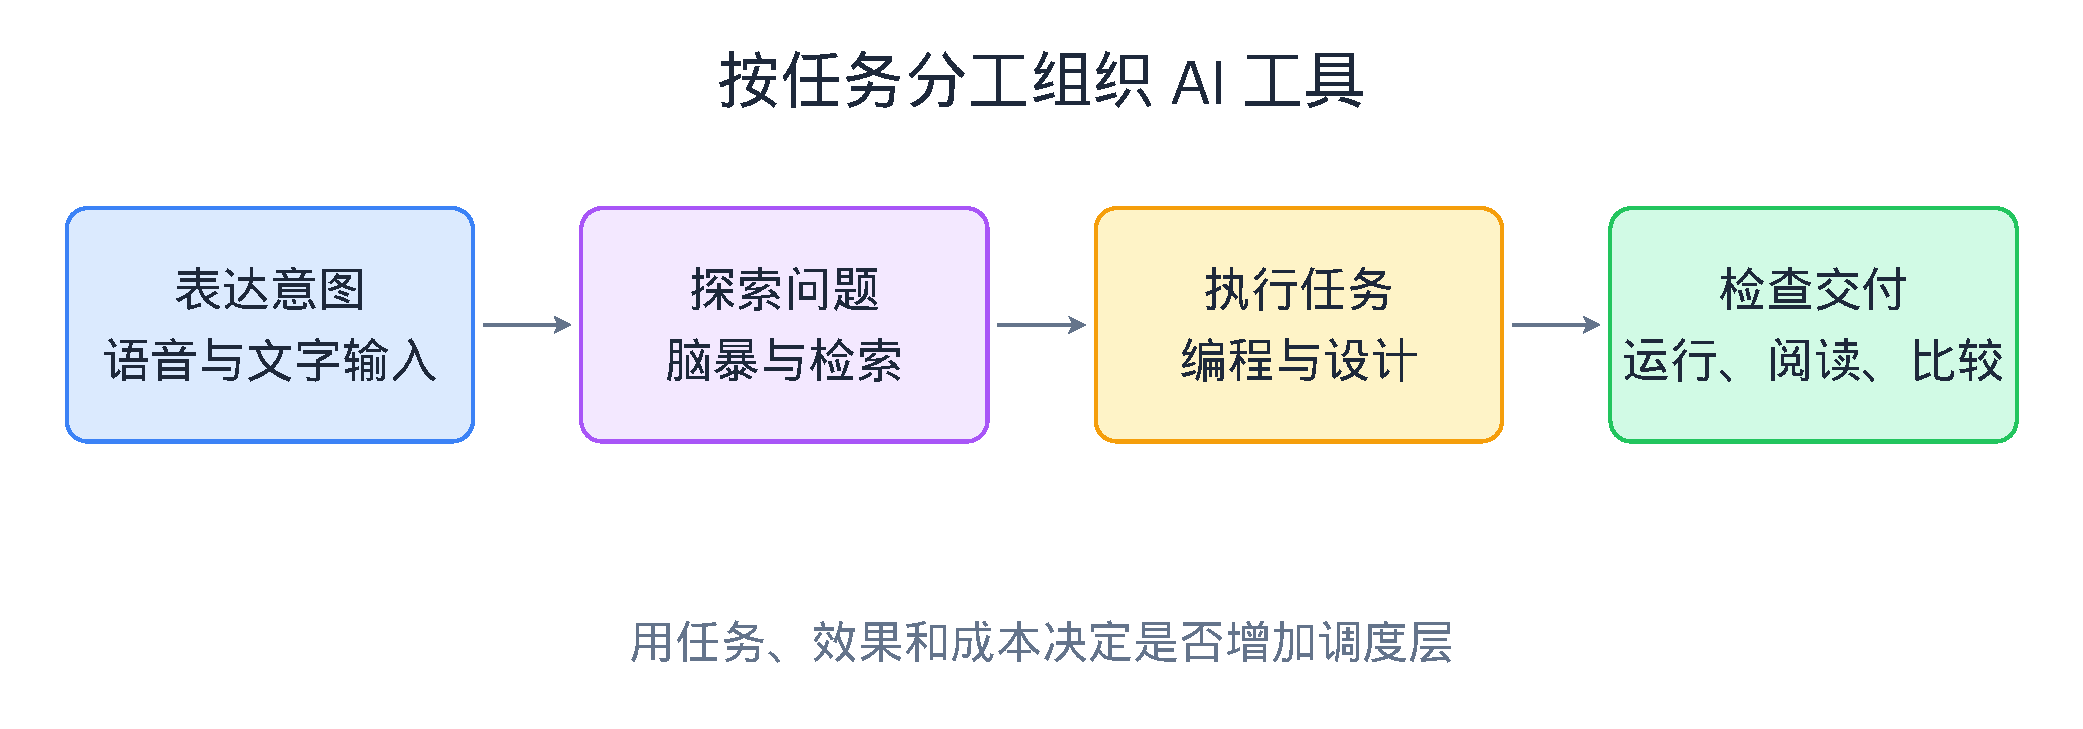
\includegraphics[width=\linewidth,height=.68\textheight,keepaspectratio]{assets/tool-workflow.pdf}
\caption{按任务分工组织 AI 工具（46:38–59:46，依据节目口述整理的机制示意图）}
\end{figure}
\begin{knowledgebox}{读图：从工具清单到个人工作流}
图面由左向右以单链实线箭头串联四个任务角色方框：第一栏是“表达意图：语音与文字输入”，如用 Typeless 将口头想法转为规整的书面提示词；第二栏是“探索问题：脑暴与检索”，对应前期发散思路或用 Manus 收集信息；第三栏是“执行任务：编程与设计”，交给 Claude Code、Codex 或画布工具完成具体产出；第四栏是“检查交付：运行、阅读、比较”。图底标注提示“用任务、效果和成本决定是否增加调度层”。
\end{knowledgebox}
顺着这一任务角色链条来看，使用者既可以根据自身习惯决定是否引入 OpenClaw 这类调度工具，也可以在“探索问题”与“执行任务”之间灵活切换记忆开关，让不同特长的模型各司其职。
\needspace{6\baselineskip}\subsection{本章小结}
本章梳理了三位嘉宾如何将零散的 AI 产品整合为个人工作流：
\begin{enumerate}
\item \textbf{按环节拆解工具}：用语音结构化工具处理输入，用专门的画布、工作流或生成式 UI 工具做探索，再交给编程代理执行；
\item \textbf{按需选择调度方式}：可根据任务复杂度与 API 成本，决定是用 OpenClaw 做统一编排层，还是手动在 Manus、Claude Code 等封装工具间切换；
\item \textbf{管理配额与记忆边界}：通过维护本地进度文档（如 \texttt{progress.md}）实现跨工具接力，并通过分离“开启记忆的脑暴模型”与“关闭记忆的执行模型”来避免信息茧房。
\end{enumerate}
\needspace{8\baselineskip}\section{工具用得越熟，越要看清自己的能力}
前面梳理了三位大学生如何将对话模型、语音输入与开发工具组合成日常工作流。当工具承担了越来越多执行环节，新的问题随之出现：AI 究竟把专业基础打得更牢，还是掩盖了能力短板？本章结合心理学研究课题、封面设计、代码排错与断网假设，讨论在重度使用工具时如何检验自身的基础与独立解决问题的能力。
\needspace{6\baselineskip}\subsection{基础决定怎样发现新问题}
在建立起多模型配合的工作流并管理好记忆上下文之后，主持人泓君向侯泰羽（Kolento）提出了一个关乎学习本质的问题：在日常专业课学习中，AI 究竟让专业基础打得更扎实了，还是削弱了基础？这个问题把讨论从工具调用技巧拉回到了学习者自身的认知变化上。

Kolento 从两个层面回应了这一问题（00:59:58–01:00:59）。第一个层面是应试效率：AI 充当了随时给出及时反馈的个性化辅导老师，让他花更少的时间拿到了更高的考试分数。第二个层面则是跨界问题的探索：在纽约大学应用心理学专业课提供的知识框架上，AI 帮他把对世界的好奇延伸到了心理学与技术结合的新问题上。

他在期末论文中尝试探索心理学的\textbf{依恋类型}（Attachment Styles，指个体在人际互动中形成的回避型、焦虑型或安全型等关系模式）是否会迁移到人与 AI 的互动中。传统心理学主要在人与人之间讨论依恋关系，而他产生了一个研究问题：当 AI 在交互中充当类似人的角色时，一个人原本对他人表现出的依恋类型，会不会同样影响他使用 AI 的模式以及他与 AI 角色建立的关系？围绕这个自己提出的课题，他在 AI 的辅助下完成了期末研究与论文写作（注：这是 Kolento 在访谈中分享的课程研究问题与探索过程，节目中未给出经证实的心理学结论）。在这里，专业课程提供了“依恋类型”这一概念框架，而工具则辅助他将这一概念投射到新场景中进行探索。

\needspace{6\baselineskip}\subsection{审美与排错依靠什么}
除了用专业概念提出新问题，在没有统一标准答案的设计与工程实践中，人的基础功底同样深刻影响着 AI 产出的质量。泓君用《硅谷101》团队制作视频封面图的日常经验做了具体说明（01:01:01–01:02:54）。尽管生成式工具已经能做出漂亮的封面图，团队依然聘请专业设计师，并且不管设计师是否使用 AI。就她的日常观察而言，一个优秀设计师自己做出好图的能力，与他用 AI 做出好图的能力是成正比的。

这种正相关源于审美与设计技巧的长期积累。泓君指出，团队可以口头告诉一个人某个位置要放什么元素，却无法在短期内教会一个人审美——有时候仅仅是字体排版上的一点点微调，在最终视觉呈现上就会拉开很大差距。如果使用者缺乏审美与设计基础，即便拿到了同样的作图工具，当工具生成的结果出现瑕疵时也无法识别，更无法通过具体指令把工具引导到更高的品味上去。她由此追问三位嘉宾：在高频使用工具后，自己底层的\textbf{元认知}（Metacognition，指人对自身认知过程、理解深度与判断标准的觉察和调控能力）究竟变强了还是变弱了？

饶杰武（Jack）结合编程实践回应了这种把关能力的重要性（01:02:55–01:04:09）。他认为在课程学习上，AI 帮他更快抓到了事物的本质；但在实际编程特别是代码量较大的项目中，模型依然会犯让人匪夷所思的错误。例如他用 Gemini 写代码时，遇到过模型在改动几十行代码时竟然漏写括号的情况；还有些时候，本来应该直接把旧版代码替换掉，模型却非要保留旧代码、新写一段代码并额外加出一个分支。Jack 强调，在 \textbf{Vibe Coding} 中，如果开发者对代码不够熟悉，任由 AI 自由发挥，写出来的程序逻辑就会非常奇怪。正如客户不在乎设计师用手绘还是用 AI、只在乎最终交付物好不好一样，无论是设计师改图还是开发者写代码，都必须在关键节点上亲自识别问题并纠正方向。

\needspace{6\baselineskip}\subsection{效率快感、学习乐趣与备用路径}
当日常执行越来越依赖人机协作，一旦工具额度耗尽或被突然抽离，工作与学习会受到什么影响？三位嘉宾都坦言自己有不同程度的“AI 上瘾”，但拆开来看，每个人对上瘾的描述、对能力被侵蚀的担忧以及脱离 AI 后的应对方式有着明显差异（01:04:10–01:12:12）。

\begin{itemize}
\item \textbf{Kolento（执行与学习双重依赖）}：他形容没有 Claude 就像电脑断网一样难受，因为 AI 承担了他约 70\% 的快速执行与 30\% 的灵感来源；一旦额度用尽，这两部分同时受阻。同时他也不把工作和日常完全分开，平时出于好奇心想学习或探索复杂问题时，就用语音输入大段杂乱的想法，期待模型给出背后的洞察（Insight），这被他称为“学习上瘾”。由于从上大学第一天起就在用 AI，他直言如果完全脱离 AI，自己现在无法直接写代码。
\item \textbf{Alfred（全天共存与人的职责反思）}：他的日常从让 OpenClaw 在 Google Calendar 排日程、读 Gmail 写回复草稿，到用 Claude Code 开发程序，全天与 AI 共存。他认为上瘾感源于省去了很多痛苦思考与左右互搏的过程，并获得了创造出原本无法想象的产物的快感；但他读完尤瓦尔·赫拉利《智人之上》（Nexus）后也担忧人的部分能力被侵蚀，因此借控制论学者诺伯特·维纳在《人有人的用处》中的观点提醒自己，要把精力放在\textbf{提出正确问题}、\textbf{进行价值判断}和\textbf{承担最终责任}这三项基础与元认知能力上。他在高中毕业后的半年闲暇里只学过通用 Python，认为完全抽离 AI 后很难开展现在正在做的开发工作。
\item \textbf{Jack（效率快感与次优备用方案）}：他把 AI 视为纯粹的效率工具，很少用于娱乐陪伴；他举例形容这种快感——当看到一件原本要花 10 小时完成的事现在半小时就能做完，省下的 9.5 小时可以自由支配，就会觉得非常爽快；编码时让 Claude Code 先生成几个 HTML 方案、把文字变成直观的图形界面（GUI），也让他感到豁然开朗。但与前两位不同，他在 2018 至 2019 年（读大学及 ChatGPT 出现之前）就已经接触写代码，因此如果 Claude Code 断掉 24 小时，他虽然难受，却仍能退回 Stack Overflow（程序员常用的技术问答社区）和早期静态网站文档，用自己经历过的次优方案继续写代码或独立写论文。
\end{itemize}

三位嘉宾的经历差异表明，工具带来的提速快感与探索乐趣是普遍的，而面对工具中断时的反应则与个人过往的学习路径密切相关。与其在抽象层面焦虑能力退化，学习者不如结合自身正在推进的课程或项目，从提问、审美排错、时间分配与备用方案四个维度定期做一次自我检查。

\begin{importantbox}{用“抽离测试”检验自己的能力结构}
判断自己是在驾驭工具还是单纯依赖工具，可以做一次思想或实操上的抽离测试：
\begin{enumerate}
\item \textbf{识别任务中的关键纠正点}：在设计排版或代码合入时，你能否一眼看出模型漏掉的括号、冗余的分支或失衡的字距？
\item \textbf{检查是否存在次优备用路径}：假设核心工具停服 24 小时，你是完全停工，还是能退回官方文档、问答社区（如 Stack Overflow）或手写草稿继续推进？
\end{enumerate}
\end{importantbox}
\begin{knowledgebox}{维纳《人有人的用处》中的三项人类职责}
Alfred 引用控制论创始人诺伯特·维纳在 20 世纪中叶著作《人有人的用处》中的观点，指出当自动化工具承接大量执行环节后，人的核心用处集中在三个无法外包的环节：
\begin{itemize}
\item \textbf{提出正确的问题}：利用学科认知定义研究或工程方向。
\item \textbf{进行价值判断}：在多个看似合理的候选方案中做出取舍。
\item \textbf{承担最终责任}：对交付物的质量、伦理与后果负责。
\end{itemize}
\end{knowledgebox}
\begin{table}[H]\centering\small
\caption{重度使用 AI 时的能力检验与个人差异对照}
\begin{tabular}{>{\raggedright\arraybackslash}p{\dimexpr(\linewidth-6\tabcolsep)/3\relax}>{\raggedright\arraybackslash}p{\dimexpr(\linewidth-6\tabcolsep)/3\relax}>{\raggedright\arraybackslash}p{\dimexpr(\linewidth-6\tabcolsep)/3\relax}}
\toprule
检验场景或人物 & 观察到的具体现象 & 对应的能力要求或应对方案\\\midrule
应用心理学期末研究（Kolento） & 将人际“依恋类型”迁移提问到人机关系 & 依靠专业课概念框架提出跨界研究问题\\[4pt]
视频封面图设计（泓君观察） & 手绘好图的能力与用 AI 出好图的能力成正比 & 凭长期积累的排版与审美微调并引导工具\\[4pt]
大代码量项目开发（Jack） & 模型漏写括号，或保留旧代码乱加新分支 & 熟悉代码逻辑，拒绝盲目放任，手动纠偏\\[4pt]
工具断供 24 小时（Kolento / Alfred） & 大学起伴随 AI 或仅学过基础 Python，开发难以推进 & 区分灵感与执行依赖，警惕底层能力被侵蚀\\[4pt]
工具断供 24 小时（Jack） & 2018–2019 年已学编程，可退回 Stack Overflow 查文档 & 保留不依赖 AI 的次优工作方案与基本功\\[4pt]
\bottomrule\end{tabular}\end{table}
当日常开发、论文写作甚至日程管理都与 AI 紧密绑定，我们很容易把工具的顺畅输出误认为自身能力的提升。结合第六章关于心理学跨界提问、封面审美、代码排错以及断网假设的讨论，下图整理了四个用于日常自我检查的问题。
\begin{figure}[H]\centering
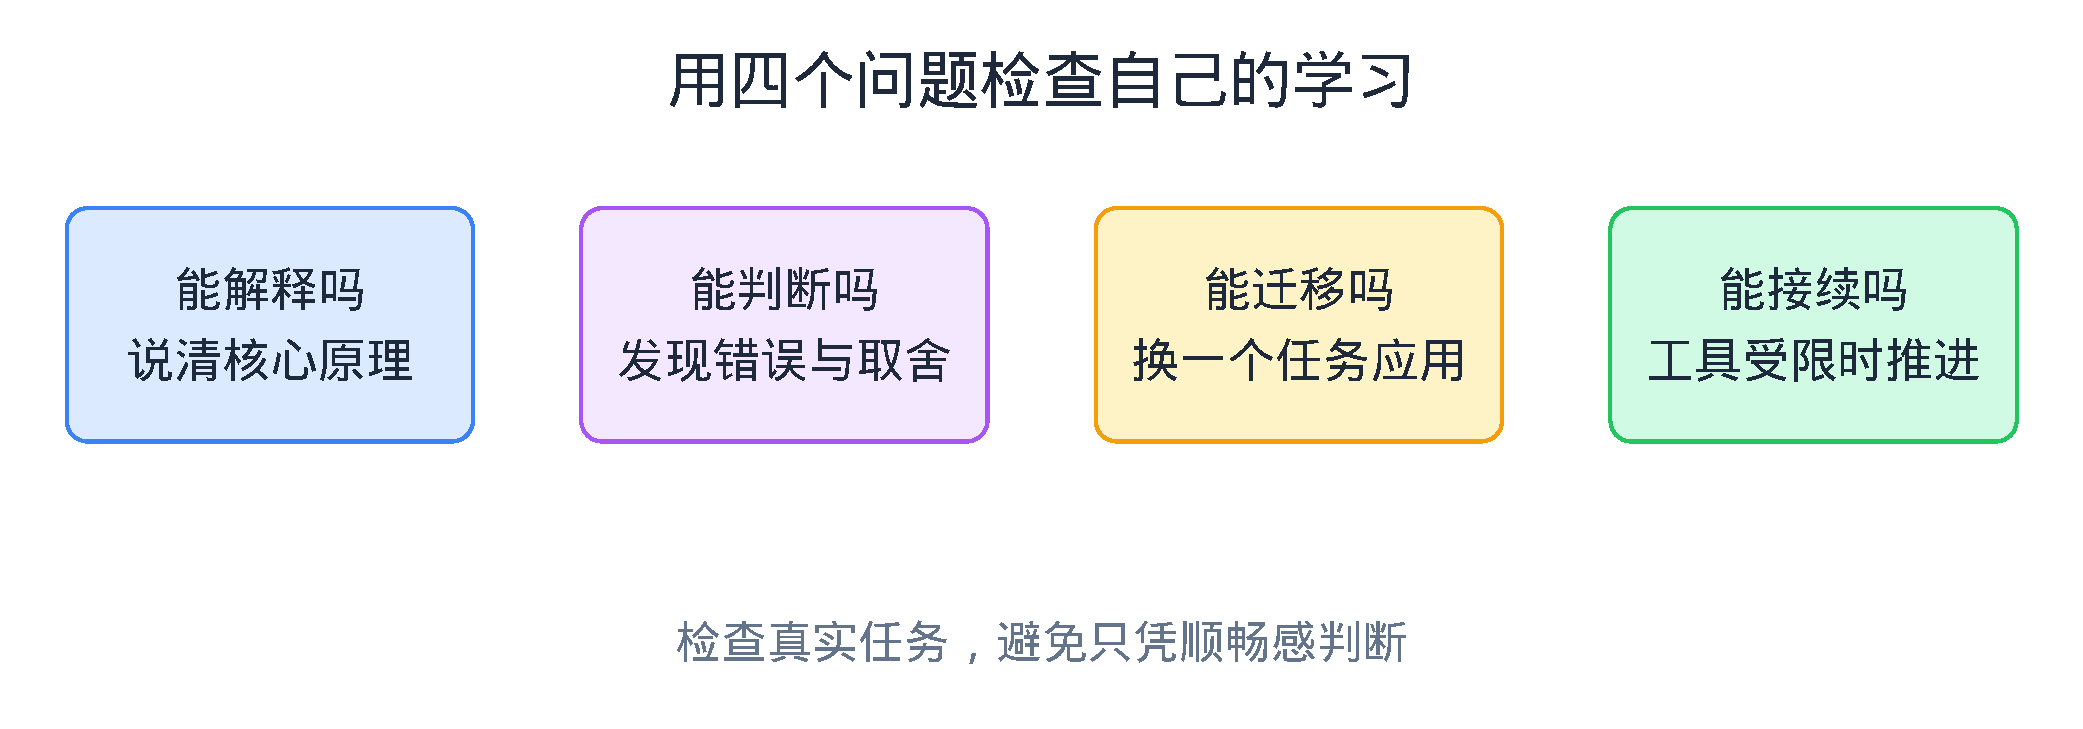
\includegraphics[width=\linewidth,height=.68\textheight,keepaspectratio]{assets/ability-check.pdf}
\caption{用四个问题检查自己的学习（59:46–01:12:12，依据节目口述整理的机制示意图）}
\end{figure}
\begin{knowledgebox}{读图：工具用得越熟，越要看清自己的能力}
图中采用无箭头的四栏横向并列结构，依次列出四个自查问题：第一栏是“能解释吗：说清核心原理”，检验是否真正消化了课程概念；第二栏是“能判断吗：发现错误与取舍”，对应设计师微调排版与 Jack 排查模型漏写括号、乱加代码分支的把关能力；第三栏是“能迁移吗：换一个任务应用”，如 Kolento 将心理学依恋类型迁移到人机关系研究中；第四栏是“能接续吗：工具受限时推进”，测试配额耗尽或断网时能否靠次优方案继续工作。
\end{knowledgebox}
正如图底标注所言，“检查真实任务，避免只凭顺畅感判断”。在完成一门课程或一个项目后，拿这四栏问题逐一对照，能帮我们看清哪些能力已经内化，哪些基本功还需要及时补齐。
\needspace{6\baselineskip}\subsection{本章小结}
\begin{enumerate}
\item \textbf{概念基础决定提问高度}：扎实的学科概念（如心理学依恋类型）能帮人在 AI 辅助下发现跨领域的新研究问题。
\item \textbf{审美与代码功底决定交付下限}：无论是封面排版微调还是排查模型漏写的括号与冗余代码分支，都需要人具备识别错误并纠正方向的基础能力。
\item \textbf{警惕工具依赖并保留备用路径}：提速与创造的快感容易让人产生工作与学习上瘾，平时应有意识训练提问、判断与兜底能力，保留脱离工具时的次优执行方案。
\end{enumerate}
\needspace{8\baselineskip}\section{用真实产出检验学习与选择}
前文探讨了如何防止工具依赖侵蚀审美、排错与独立推进的能力。当工作流搭建完毕，我们该如何客观评估 AI 带来的真实收益？本章从实证实验与记者工作经验出发，剖析为何主观提速感会掩盖整条链路的校验成本；接着结合毕业季的求职与创业选择，说明如何靠真实项目沉淀职业判断，并对比更年轻一代对技术共处的不同理解。
\needspace{6\baselineskip}\subsection{为什么感觉更快，实际却可能更慢}
在前一章，三位嘉宾都谈到了使用 AI 推进工作和学习时的爽快感。但这种不断获得即时反馈的主观体验，是否必然意味着整项任务的实际完成速度变快了？侯泰羽（Kolento）在访谈中分享了评估机构 METR（Model Evaluation \& Threat Research，模型评估与威胁研究机构）于 2025 年发布的一项随机对照实验（01:12:20–01:13:15）。该研究测试了 2025 年早期的 AI 工具（主要为 Cursor Pro 配合 Claude 3.5/3.7 Sonnet）：实验邀请了 16 位有多年开发经验、且高度熟悉自身大型开源代码库的资深开发者，随机分配了 246 个真实仓库任务，一半允许使用 AI，一半禁止使用。最终测量结果与直觉相反：允许使用 AI 的任务，实际完成耗时反而增加了 19\%；然而在实验开始前开发者预期 AI 能提速 24\%，甚至在亲身经历减速、实验结束之后，受试开发者依然主观估计 AI 让自己提速了 20\%。

为什么主观感知的提速与客观测量的耗时会出现反向落差？Kolento 在分享中将这一现象概括为“生产力安慰剂”：AI 的即时反馈让人产生了正在飞速前进的幻觉，但在主观评估时，人们往往漏算了验证、调试和返工所消耗的隐性时间。他还顺着这一结果提出了自己所称的“资深悖论”（Seniority Paradox）：在他看来，资深专家已经建立了高度优化的工作流，AI 泛化的建议对他们可能形成干扰噪音；而初学者则可以把 AI 当作全天候老师，用来快速填补语法和设计模式上的空白。需要严格区分的是，METR 的这项随机对照实验仅测试了熟悉自身代码库的资深开发者，并未设立初学者对照组（“生产力安慰剂”与“资深悖论”也是嘉宾对实验启发的概括，而非 METR 报告的官方术语）；关于新手受益、脱离电脑或 Excel 也无法直接工作的类比，属于 Kolento 结合自身零基础学习体验所做的延伸思考（01:12:50–01:14:09）。

主播泓君从自己的新闻从业经历中，为这种“局部提速但整体未快”的机制提供了另一个具体的印证（01:14:10–01:15:12）。她刚来美国做记者时，面对英文采访录音，需要自己一边听、一边逐字敲下英文，再翻译成中文并精简成稿。后来有了自动语音转文字和 AI 翻译工具，看似省去了繁琐的听打环节，但她实际核算整篇文章的交付时间时，发现新旧两种方式的总耗时差不多，甚至有时自己从头逐字听打反而更快。原因在于，手工听打并不是纯粹的机械劳动——在听录音和敲字的过程中，她的大脑已经在同步思考文章的叙事节奏，并判断哪些段落需要删减；而如果直接拿到一份机器转写并翻译好的长文本，她反而要额外花大量时间去核对事实、寻找错误漏洞并重新梳理结构。这说明检验工具是否提效，不能只看生成初稿的那几秒钟，而要把核查、删改和消化的完整链路耗时一起算进去。

\needspace{6\baselineskip}\subsection{从短期尝试形成职业判断}
在工具收益需要全链路核算的同时，这批与生成式 AI 共同度过大学时光的学生在走向社会时，也面临着剧烈变动的外部环境。林桐宇（Alfred）感到，无论是技术演进还是社会文化与政治经济环境，未来的变化都很难靠过往经验做简单的线性外推。在难以预知远期终局的混沌状态下，个人除了保持底层的学习能力，更需要依靠内心的坚定信念（conviction 与 belief）去适应环境（01:15:12–01:16:33）。

到了节目录制所在的求职与毕业季，Kolento、饶杰武（Jack）和 Alfred 都倾向于直接创业，并在各自的求职投递或身边同学中观察到了不同的现实处境（01:16:33–01:18:47）：
\begin{itemize}
\item \textbf{岗位门槛与竞争转移（Kolento 的看法）}：他认为求职者并不是直接被 AI 替代，而是被更擅长用 AI 的人替代；当越来越多人会使用 AI 时，企业招聘的门槛也随之变高。
\item \textbf{企业评估标准模糊（Jack 的投递体会）}：Jack 在实际投递简历的过程中感受到，虽然大家都在提找“会用 AI 降本增效”的人才，但无论对申请者还是企业端而言，对于如何界定和衡量“会使用 AI 的人才”都还缺乏统一、清晰的标准。
\item \textbf{身边同学的求职分化（Alfred 的局部观察）}：Alfred 看到自己身边的法学院同学找一份与三年前相同的工作（如律所、企业法务或竞争更激烈的公检法岗位）困难了许多，不少人因此思考向有增量的 AI 行业转型；同时据他在美国的观察，一些计算机背景的毕业生因为北美大厂冻结软件开发工程师（SDE）招聘名额而面临就业困难，转而把去创业公司找工作视为主要的希望。
\end{itemize}

在企业衡量标准尚不清晰的情况下，空泛宣称“会用 AI”很难建立优势，真正能支撑个人选择的依然是提前积累的真实产出。Alfred 表示自己之所以在求职或创业时没有遇到太大困境，是因为他在过去两年里全情投入（all in），把看论文、学代码和做项目完整地实践了一遍，积累了五六个实际项目经验。这种在短期内密集尝试的做法，也帮他在两三年前就明确排除了从事法律相关职业的可能，并将自己未来的大方向确立为“解放”（Emancipation）——即探索如何借助技术进步让人们在获得基础生活保障的同时，从繁重的工作中解放出来，去做真正喜欢且愉悦的事（01:17:28–01:19:28）。

\needspace{6\baselineskip}\subsection{下一代如何理解与 AI 共处}
当三位受访大学生还在认真复盘“如果抽离 AI，自己有哪些事做不了”时，更年轻一代的学习者又是如何看待人机关系的？在这期节目于 2026 年 2 月录制完成后，泓君偶然参加了一场硅谷高中生的聚会，并把访谈中“最早用 AI 学编程的大学生离开 AI 后反而不会手写代码”的现象抛给了现场的高中生（01:19:40–01:20:49）。

出乎意料的是，现场一位比受访大学生年轻三四岁的高中生立刻反驳了这个问题本身。在那个高中生看来，“如果离开 AI 怎么办”是一个根本不成立的伪命题——这就好比父母辈是电视的原住民，年轻一代是智能手机的原住民，而今天已经没有人会去严肃讨论“如果明天没有手机了你该怎么生活”。这群高中生甚至直接认为，凡是 AI 已经掌握的技能，他们就不再需要花时间去学了。

把那场聚会中硅谷高中生的直接反应，与节目里三位大学生的复盘放在一起，可以看到两种不同切入点的理解：聚会中的高中生将 AI 视为像智能手机一样不会离开的默认前提，认为 AI 已经会做的事就不必再学；而访谈中的三位大学生，无论是经历过 AI 出现前手写代码的 Jack，还是从大一就开始借助 AI 跨界学编程与做产品的 Alfred 和 Kolento，都在高频使用工具的实践中深切体会到需求拆解、代码排错、审美把关与价值判断的分量。正如泓君在节目尾声所总结的，关于“什么是有用的知识、什么是不可替代的能力”，是新时代向每一个人发出的共同考卷，而这批大学生只是最先交卷回答的那几个人。无论技术环境如何演进，核算完整任务链路的真实产出，并在选择中保留人的判断与责任，始终是应对这份考卷的扎实支点（01:20:31–01:21:25）。

\begin{importantbox}{评估效率要算“全链路总账”}
单点生成速度不等于完整任务的交付效率。在工作流中引入 AI 时，真实耗时由两部分相加：
\begin{itemize}
\item \textbf{生成时间}：向模型输入需求并获得初稿或候选代码的时间。
\item \textbf{检验与返工时间}：事实核查（Fact-check）、阅读理解他人/机器逻辑、调试报错及删改重构的时间。
\end{itemize}
当人工原生的执行过程（如记者边听打边构思、资深程序员按既定架构编码）已经将“思考与校验”内嵌在动作中时，外挂 AI 生成反而可能因为打断心流或增加排错负担，导致全链路总耗时上升。
\end{importantbox}
\begin{warningbox}{注意区分实验边界与延伸推论}
引用实证研究时，需对齐实验的受试样本与变量：
\begin{itemize}
\item \textbf{METR 2025 早期实验}：受试者为 16 位有多年经验、熟悉自身开源仓库的开发者，共 246 个任务；结果是允许用 AI 的任务实际完成耗时增加 19\%，而实验后受试者仍主观估计提速 20\%。
\item \textbf{嘉宾的延伸思考}：该实验未设置初学者对照组。将新手受益与专家减速对比的“资深悖论”，属于 Kolento 结合个人学习体验提出的延伸解释。
\end{itemize}
\end{warningbox}
\begin{table}[H]\centering\small
\caption{工具提效感与真实产出的检验对照}
\begin{tabular}{>{\raggedright\arraybackslash}p{\dimexpr(\linewidth-6\tabcolsep)/3\relax}>{\raggedright\arraybackslash}p{\dimexpr(\linewidth-6\tabcolsep)/3\relax}>{\raggedright\arraybackslash}p{\dimexpr(\linewidth-6\tabcolsep)/3\relax}}
\toprule
工作与决策场景 & 常见的表面感知或口号 & 基于真实产出的检验机制\\\midrule
资深开发者修复开源库任务 & 模型秒出代码，主观感觉提速 20\% & 计入阅读、调试与返工后，METR 实验测量实际耗时增加 19\%\\[4pt]
记者整理英文采访并成稿 & 语音转写加机器翻译省去打字时间 & 手工听打同步完成了构思与删减，机器初稿反而增加核查负担\\[4pt]
求职者证明自身 AI 能力 & 在简历中泛泛宣称熟练使用各类 AI 工具 & Jack 观察到企业缺乏统一评估标准；Alfred 靠提前积累的读论文、写代码与项目产出建立优势\\[4pt]
学生规划长期职业方向 & 按入学专业线性外推或做僵化的远期预设 & 通过短期密集的论文、代码与产品试错，确认真实兴趣与能力边界\\[4pt]
\bottomrule\end{tabular}\end{table}
为什么人们在用 AI 写代码或转写稿件时常常觉得飞快，实际结项时却可能耗时更长？结合 Kolento 分享的 METR 随机对照实验与泓君早年做英文采访记者的写稿经历，下图将效率评估放回完整的任务链条中。
\begin{figure}[H]\centering
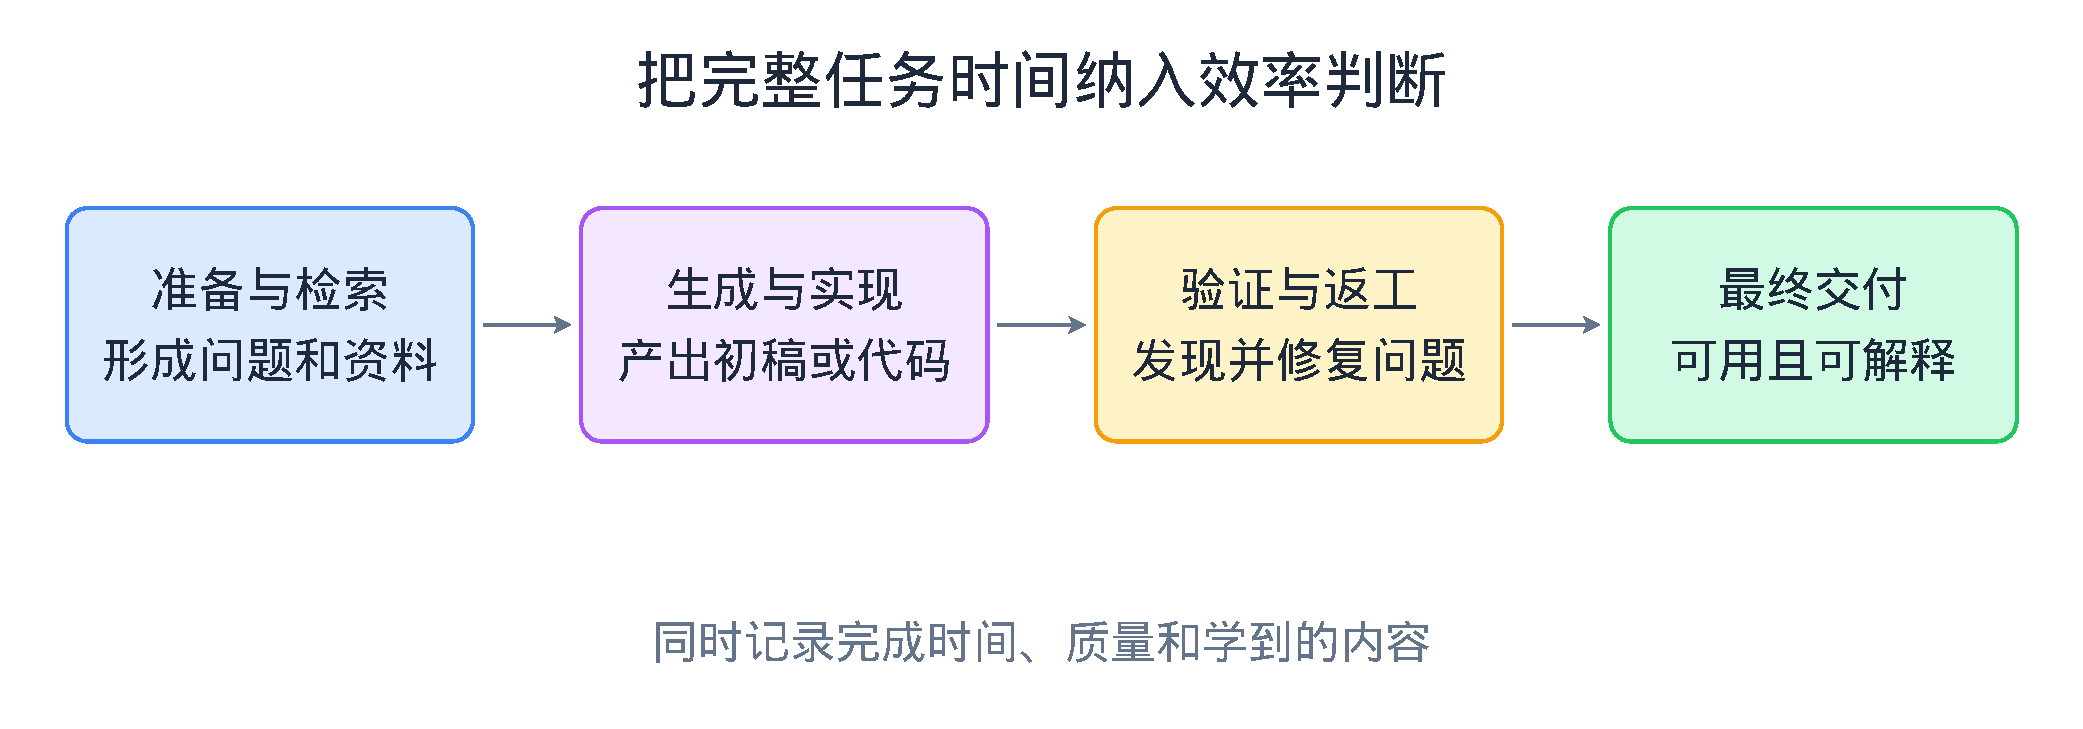
\includegraphics[width=\linewidth,height=.68\textheight,keepaspectratio]{assets/whole-task.pdf}
\caption{把完整任务时间纳入效率判断（01:12:12–01:15:21，依据节目口述整理的机制示意图）}
\end{figure}
\begin{knowledgebox}{读图：用真实产出检验学习与选择}
请顺着图中从左到右的单链实线箭头依次阅读四个阶段：第一栏是“准备与检索：形成问题和资料”；第二栏是“生成与实现：产出初稿或代码”，这也是人们主观感受AI提速最明显的环节；第三栏是“验证与返工：发现并修复问题”，涵盖事实核查、调试报错与结构删改；第四栏是“最终交付：可用且可解释”。图底文字提示“同时记录完成时间、质量和学到的内容”，引导读者核算从准备到交付的全过程。
\end{knowledgebox}
把这四个阶段连起来算总账就能看清：当机器加快了第二栏“生成与实现”的速度，却把大量工作转移到第三栏“验证与返工”时，整项任务的实际完成时间未必缩短。只有综合考量四步的总耗时与交付质量，才能做出清醒的工具取舍。
\needspace{6\baselineskip}\subsection{本章小结}
本章从真实产出的角度检验了 AI 时代的学习与职业选择：
\begin{enumerate}
\item \textbf{警惕生产力安慰剂}：METR 实验与记者写稿经验表明，局部的生成提速常被核查、调试与重构的隐性成本抵消，评估工具收益必须核算全链路时间。
\item \textbf{用具体作品应对求职分化}：面对传统岗位收缩与招聘标准模糊，持续跑通真实项目比口头宣称“会用 AI”更有说服力。
\item \textbf{在共处中保留判断力}：更年轻一代已将 AI 视为默认基础设施，但无论是否假设“离开 AI”，对最终产出负责的审美、排错与价值选择始终无法外包。
\end{enumerate}
\needspace{8\baselineskip}\section{总结与延伸}
纵观三位名校生的求学与实践轨迹，AI 对大学教育的冲击并未消解学习的意义，反而迫使学习者将外在技能训练与内在价值判断剥离开来。无论是 Alfred 用 30\% 公开课打底配合 70\% 追问与项目复盘、并在脱离工具的现场手写考试中检验法律论证链，还是 Kolento 以トップ作品为锚点寻找关键区分点、靠原始链接与真人专家双路校准，抑或 Jack 在高频让 AI 参与作业流程时坚持亲自拆解需求与筛选方案，都指向同一条底线：工具可以承接检索、生成与执行，但提出问题、评估优劣与承担最终责任始终落在人身上。

在延伸思考中，学习者可以从三个维度持续审视自己的工作流：第一，把单次生成的爽快感放回包含核查、排错与重构的完整任务链路中核算真实耗时，警惕“生产力安慰剂”；第二，在组合语音输入、通用编排与垂直代理时，合理隔离脑暴记忆与干净执行上下文，并预留脱离特定工具后的次优兜底方案；第三，跳出固定课表的线性预设，在哲学阅读、跨界课题与短期高频的真实项目交付中锤炼审美与信念。面对技术演进向每一代人发出的共同考卷，唯有把外部工具转化为内化的理解深度与独立的取舍标准，才能在剧烈变动的环境中站稳脚跟。
\subsection{拓展阅读}
以下资料供回看节目、查阅术语与继续学习。
\begin{itemize}
\item 硅谷101：完整节目：\url{https://www.bilibili.com/video/BV1zD5a6bEoY/}
\item METR：2025年早期AI对资深开源开发者生产率的研究：\url{https://metr.org/blog/2025-07-10-early-2025-ai-experienced-os-dev-study/}
\end{itemize}
\end{document}
